\documentclass[aspectratio=169,11pt]{beamer}

% ----------------------------------------------------------------------
% Theme
% ----------------------------------------------------------------------

\usetheme{default}
\usecolortheme{default}

% Remove navigation symbols
\setbeamertemplate{navigation symbols}{}

% ----------------------------------------------------------------------
% Packages
% ----------------------------------------------------------------------

\usepackage[T1]{fontenc}
\usepackage{lmodern}

\usepackage{amsmath,amssymb,amsthm,amsfonts}
\usepackage{bbm}
\usepackage{booktabs}
\usepackage{graphicx}
\usepackage{hyperref}

\usepackage{listings}
\usepackage{xcolor}

\hypersetup{
  colorlinks=true,
  urlcolor=structure.fg,
  linkcolor=structure.fg,
  citecolor=structure.fg
}

\lstset{
  language=C,
  basicstyle=\ttfamily\small,
  keywordstyle=\color{blue},
  commentstyle=\color{green!60!black},
  stringstyle=\color{red},
  numbers=left,
  numberstyle=\tiny,
  frame=single,
  breaklines=true
}

% ----------------------------------------------------------------------
% Metadata
% ----------------------------------------------------------------------

\title{{APMAN}}
\author{Fran\c cois Cayre, Auguste Olivry}
\institute{Phelma / 2A {SEOC}}
\date{2026--2027}

% ----------------------------------------------------------------------
% Footer
% ----------------------------------------------------------------------

\setbeamertemplate{footline}{
    \leavevmode
    \hbox{
        \begin{beamercolorbox}[wd=.30\paperwidth,ht=2.5ex,dp=1ex,leftskip=1em]{author in head/foot}
            \insertshortauthor
        \end{beamercolorbox}

        \begin{beamercolorbox}[wd=.50\paperwidth,ht=2.5ex,dp=1ex,center]{title in head/foot}
            \insertshorttitle
        \end{beamercolorbox}

        \begin{beamercolorbox}[wd=.20\paperwidth,ht=2.5ex,dp=1ex,rightskip=1em]{date in head/foot}
            \insertframenumber{} / \inserttotalframenumber
        \end{beamercolorbox}
    }
}

% No headline
\setbeamertemplate{headline}{}

% ----------------------------------------------------------------------
% Outline at beginning of each section
% ----------------------------------------------------------------------

\AtBeginSubsection[]
{
  \begin{frame}<beamer>{Outline}
    \tableofcontents[
      currentsubsection, 
      hideothersubsections, 
      subsectionstyle=show/shaded/hide
    ]
  \end{frame}
}

% ----------------------------------------------------------------------
% Document
% ----------------------------------------------------------------------

\begin{document}

% ----------------------------------------------------------------------
\begin{frame}
    \titlepage
\end{frame}


% ----------------------------------------------------------------------
\begin{frame}[fragile]{Course objectives}

  \begin{enumerate}
  \item To tackle real-world issues in programming, testing and benchmarking
  \item To learn (quite) a few techniques in C

    Modules, genericity, iterators, meta-programming, generalization/specialization
  \item To understand how a streamlined methodology brings {\em guarantees} to your code
  \item To master complexity issues---in (applied) Computer Science {\em and} with experiments
  \item To understand (and close!) the gap between the textbook and robust, fast code
  \end{enumerate}

  You are given an environment that implements much of what these slides discuss:
  \begin{itemize}
  \item It's only good news on a higher level: that's a lot of real, {\em hardcore} C to digest.
  \item These slides describe the techniques we used as independently as possible.

    Sections ``Setting the stage'' and ``Basic tools for data structures.''
  \item Ask yourself/us how to make the most out of it! With the least effort!
  \end{itemize}
  
\end{frame}


% ======================================================================
\section{Hashing (for data indexing)}

% ======================================================================
\subsection{A subjective history of {\em ``Where did I put the damn keys?''}}

% ----------------------------------------------------------------------
\begin{frame}[fragile]{Searching, by hand}

  Earliest alternative to linear search: hand-built index
  \begin{itemize}
  \item Mesopotamia

    Clay tablets organized in collections, lexical catalogues constructed {\em systematically}.

  \item Ancien Egypt

    Administrative records by category, scribes produce {\em ordered} word (and sign) lists.

    \begin{itemize}
    \item Most often: single-level indexing
    \end{itemize}

  \item Greco-Roman world: most notable example is the Library of Alexandria
    \begin{itemize}
    \item Callimachus' {\em Pinakes}: huge catalogue by author {\em and} subject, with biblio info
    \item Likely the first known database
    \item ``Practical'' multi-level indexing
    \end{itemize}
  \item Romans credited to leverage alphabetical order for organization and search
    \begin{itemize}
    \item ``Abstract'' multi-level indexing
    \end{itemize}
  \item Pre-Google Internet had collaborative construction of curated website collections
    \begin{itemize}
    \item Still used on the Darknet today (darksites not discoverable by construction)
    \end{itemize}
  \end{itemize}

\end{frame}


% ----------------------------------------------------------------------
\begin{frame}[fragile]{Searching, with a machine}

  Main problems with an index: built by hand, logarithmic up to index depth.  

  You may still have a long list of data to check once you reached an index leaf.

  \begin{itemize}
  \item Mid-1940's: {\em Associative access} (making the goal explicit)

    K. Zuse (Germany), V. Bush (USA).
    
    {\em ``What if those strange machines allowed to {\em search data by its very contents}?''}

    \begin{itemize}
    \item Goal: automatic (non-human) scribes.
    \end{itemize}
  \item 1953: {\em Chaining hashtables} (closed addressing)

    H.P. Luhn.

    {\em ``Let's {\em compute from the data itself} the number of the list where it belongs!''}

    \begin{itemize}
    \item On an IBM 701: 2000 words of magnetic-drum memory, 72-bit machine words;
    \item Full pointers too costly: have smaller indices into storage array instead;
    \item That's basically our pointer arithmetics (to save on the pointers size.)
    \end{itemize}
  \end{itemize}

\end{frame}


% ----------------------------------------------------------------------
\begin{frame}[fragile]{Searching, with a machine of today}

  \begin{itemize}
  \item 1954: {\em Linear hashtables} (open addressing)

    G. Amdahl, E. McGraw, A. Samuel (IBM 701) + A. Ershov independently.

    {\em ``By the way, you could even have {\em implicit} lists!''}

  \item Late 1960's: The word ``hashing'' eventually becomes standard terminology
    \begin{itemize}
    \item Many variants explored: quadratic hashing, double-hashing, Cuckoo hashing, {\em etc.}
    \end{itemize}

  \item 1986: {\em Robin-Hood hashing} (minimize inequalities to maximize robustness)

    P. Celis.
    
    {\em ``Let's have a linear table {\em self-organize to maintain highest performance}!''}

    \begin{itemize}
    \item Robustness? {\em RH maintains highest performance under a larger panel of workloads.}
    \end{itemize}
    
  \item 2022: {\em SwissTable} (leverage insn-level, parallel probing)

    Abseil (company).
    
    {\em ``Let's have {\em ultra-fast SIMD lookups with metadata} control bytes!''}

    \begin{itemize}
    \item Robin-Hood on steroids (most lookups with a single probing insn)
    \item Influential design (Rust's HashBrown table, {\em etc.})
    \end{itemize}
  \end{itemize}
  
\end{frame}


% ======================================================================
\subsection{A world of complexity}

% ----------------------------------------------------------------------
\begin{frame}[fragile]{The big picture (searching)}

  Applications fall in two categories:
  \begin{enumerate}
  \item If you are only concerned with {\em exact search}, go with hashtables

    {\em ``What is the value of this key?''}

    Hashtables are unbeatable at this game (amortized constant-time)
    
  \item If you need {\em interval search}, go with ordered search trees

    {\em ``What are the keys in this interval?''} (spatial data, ecological data, {\em etc.})

    \begin{itemize}
    \item {\em Lower-bound} search primitive.
    \item The lower bound in the data may or may not be that of the search interval
    \item Easy to search for absence or presence+value of one specific key

      To instantiate exact search for comparison purposes.
    \end{itemize}
  \end{enumerate}

  That's a lot of ground to cover!
  
\end{frame}


% ----------------------------------------------------------------------
\begin{frame}[fragile]{The big picture (hashing)}

  We are {\em not} doing crypto!
  \begin{itemize}
  \item Hash data to produce secure digests (Keccak, {\em etc.})
  \item Much more stringent mathematical requirements

    Collision resistance, pre-image resistance, second pre-image resistance.
  \end{itemize}

  But we may still have adversaries:
  \begin{itemize}
  \item DoS (Denial-of-Service) attack on routers

  \item Targeted weakness was the router internal hashtable

  \item Hackers triggering catastrophic, degenerate linear-time search

    Poorly designed hash function allowed crafting the right attack sequence

  \item SipHash hash function specifically designed as a counter-measure
  \end{itemize}

\end{frame}


% ----------------------------------------------------------------------
\begin{frame}[fragile]{The big picture (hashing + searching)}

  \begin{itemize}
  \item A hash is a source of pseudo-randomness derived from the key alone.
  \end{itemize}

  Search trees may use a hash in essentially two forms:

  \begin{enumerate}
  \item Cheap and efficient randomized balancing of a BST (treap)

    More complicated and stringent balancing with AVL trees, Red-Black trees.
  \item Plain routing info inside the tree (hashtrie)

    Balancing unordered keys.
  \end{enumerate}

  It is common practice for a hash-based search structure to {\em finalize} the hash.

  The user must provide the hash function, which may be poorly designed:
  \begin{itemize}
  \item Add some internal layer of ``hashing the hash''
  \item Must be fast (a few CPU insns): \textsc{xor}-based bit-mixer, Fibonacci hashing
  \end{itemize}

  Cheap patch against entry-level contingencies, close to useless under attack.
  \begin{itemize}
  \item Gain operational reach and stability.
  \end{itemize}
  
\end{frame}




% ======================================================================
\section{Setting the stage}

% ======================================================================
\subsection{Preprocessor}

% ----------------------------------------------------------------------
\begin{frame}[fragile]{What is it?}

  \begin{itemize}
  \item Commands that (conditionnally) transform text, {\em prior to compilation}
    \begin{itemize}
    \item \lstinline{#include}, \lstinline{#if}, \lstinline{#else}, \lstinline{#elif}, \lstinline{#endif}, \lstinline{#define}, \lstinline{#ifdef}, \lstinline{#ifndef}.
    \end{itemize}
  \item Two output facilities, one to trigger failure:
    \begin{itemize}
    \item \lstinline{#warning "You have been warned"}: compilation continues after printing
    \item \lstinline{#error "teH iMPosSiBLe HaPpEneD!"}: compilation fails after printing
    \end{itemize}
  \item Two operators (your life just changed):
    \begin{itemize}
    \item \lstinline{# symbol}

      will create {\em constant string} \lstinline{"symbol"} (symbol ``stringification'')
    \item \lstinline{foo ## bar}

      will create {\em symbol} \lstinline{foobar} (symbol concatenation)
    \item One minor glitch: better used encapsulated, more later.
    \end{itemize}
  \item What is actually compiled is the output of the preprocessor.
    \begin{itemize}
    \item What about conditional copy-pastes that end up writing code for you?
    \end{itemize}
  \end{itemize}

\end{frame}

% % ----------------------------------------------------------------------
\begin{frame}[fragile]{Example}

  Crudeness of the preprocessor commands makes debugging them a little tedious:

  \begin{lstlisting}
    #include <stdint.h> /* Integers and their bounds */

    #if UINTPTR_MAX == UINT64_MAX
    #warning "64-bit pointers. Now that's a machine!"

    #elif UINTPTR_MAX == UINT32_MAX
    #warning "32-bit pointers. I like little gadgets too!"

    #else
    #error "I will refuse to compile on alien hardware"
    #endif
  \end{lstlisting}

  There's no \lstinline{printf()}-like facility nor any C construct!

  Except for (possibly parenthesized) logic/arithmetic testing with \lstinline{#if} and \lstinline{#elif}.

\end{frame}

% ----------------------------------------------------------------------
\begin{frame}[fragile]{Symbols}
  
  \begin{itemize}
  \item Preprocessor symbols may or may not be defined.
  \item When they are defined, they may or may not have a value.
    \begin{itemize}
    \item And when they have a value, it may or may not be a {\em macro}.
    \end{itemize}
  \end{itemize}

  This will eventually let us achieve C code abstraction w.r.t.
  \begin{itemize}
  \item Machine-dependent features (pointer size, SIMD extensions, {\em etc.})
    \begin{itemize}
    \item Isolate code for bleeding-edge hardware, preserve safe fallback for production.
    \end{itemize}
  \item Lower-level implementation choices:
    \begin{itemize}
    \item \lstinline{set.h} $\rightarrow$ \lstinline{map.h} $\rightarrow$ \{ \lstinline{hashtable.h}, \lstinline{bst.h}, \lstinline{list.h} \}
    \item \lstinline{set.h} will essentially build on \lstinline{put()}/\lstinline{get()} from \lstinline{map.h} to implement union, membership testing, symmetric difference, {\em etc.}

      Any other structure providing \lstinline{put()}/\lstinline{get()} could be used.
    \item \lstinline{map.h} will factor out all possible code so the core algorithmic differences are isolated in \lstinline{list.h}, \lstinline{bst.h} and \lstinline{hashtable.h}.
    \end{itemize}
  \end{itemize}

\end{frame}

% ----------------------------------------------------------------------
\begin{frame}[fragile]{Preprocessor caveats (side-effects)}

  Suppose we have:
  \begin{lstlisting}
    #define gen_abs(x) ((x)<0?-(x):(x))
  \end{lstlisting}

  If you use it with side-effects, a kitten will die:
  \begin{lstlisting}
    int a = -3;

    int gabs = gen_abs(a++);

    /* Expands to:   int gabs = ((a++)<0?-(a++):(a++));
    
       => The value of a is now -1, yet -2 was likely expected.
    */
  \end{lstlisting}

\end{frame}

% ----------------------------------------------------------------------
\begin{frame}[fragile]{Preprocessor caveats (parentheses)}

  Suppose we have:
  \begin{lstlisting}
    #define get_idx(p) p->idx
  \end{lstlisting}

  If you use it with pointer arithmetics, a kitten will die:
  \begin{lstlisting}
    struct foo_t { int idx; };
    
    struct foo_t *arr = calloc(42, sizeof *arr);
    /* Fill arr as expected */
    int id = get_idx(arr+2);

    /* Expands to:   int id = arr+2->idx;
    
       => Syntax error.
    */
  \end{lstlisting}

\end{frame}

% ----------------------------------------------------------------------
\begin{frame}[fragile]{Preprocessor caveats (do and don't)}


  \begin{enumerate}
  \item {\em Never} use a macro with side-effects in the argument(s);
  \item Put parentheses around every parameter occurrence:
  \begin{lstlisting}
    #define get_idx(p) (p)->idx
  \end{lstlisting}
  And around the macro body itself if it's to be used inside other expressions:
  \begin{lstlisting}
    #define list_is_empty(list) ((list) == LIST_END_MARKER)
  \end{lstlisting}
  \end{enumerate}

  {\em Incipit trag\oe dia.}
  
\end{frame}

% ----------------------------------------------------------------------
\begin{frame}[fragile]{Common pattern: Arch.-dependent constants}

  Suppose the start of some \lstinline{src/list.c}:
  
  \begin{lstlisting}
    #include <stdint.h> /* Integers and their bounds */
    /* We may have other plans for NULL */
    #if   UINTPTR_MAX == UINT64_MAX
    /* Define a symbol with a constant value */
    #define LIST_END_MARKER ((void*)0xffffffffffffffffULL)
    #elif UINTPTR_MAX == UINT32_MAX
    #define LIST_END_MARKER ((void*)0xffffffffUL)
    #else
    #error "Unsupported architecture"
    #endif

    /* Define a *macro* symbol, works on 32/64-bit machines */
    #define LIST_END(list) ((list) == LIST_END_MARKER)
  \end{lstlisting}
  
\end{frame}

% ----------------------------------------------------------------------
\begin{frame}[fragile]{Common pattern: Arch.-dependent constants}

  Our \lstinline{src/list.c} may continue like:
  
  \begin{lstlisting}
    #include <stddef.h> /* size_t */

    size_t list_length(list_t l) {
      size_t len = 0;

      for ( ; !LIST_END(l) ; l = l->next)
        len++;

      return len;
    }
    
    /* Plenty of code to finish implementing lists */

    #undef LIST_END         /* Clean locally-defined symbols */
    #undef LIST_END_MARKER
  \end{lstlisting}

\end{frame}

% ----------------------------------------------------------------------
\begin{frame}[fragile]{Common pattern: Arch.-dependent constants (cont'd)}

  What the compiler will automatically get for compilation on a 32-bit machine:
  
  \begin{lstlisting}
    size_t list_length(list_t l) {
      size_t len = 0;

      for ( ; !((l)==(void*)0xffffffffUL) ; l = l->next)
        len++;

      return len;
    }
  \end{lstlisting}

  Use \lstinline{-E} compiler flag to get the preprocessor output.

  {\em Warning!} This is very verbose (all the \lstinline{#include}'d contents is there).

  You have to anticipate for the correct expansion of macros and symbol values!
  
\end{frame}
  
% ----------------------------------------------------------------------
\begin{frame}[fragile]{Common pattern: Conditional inclusion}

  Suppose a higher-level \lstinline{include/structure.h}:
  
  \begin{lstlisting}
    #if defined(TREE_STRUCT)

    #include <structure/tree.h>

    #elif defined(LIST_STRUCT)

    #include <structure/list.h>

    #else
    #error "Unsupported/unspecified data structure"
    #endif /* TREE_STRUCT, LIST_STRUCT */

    /* Common code for all data structures */
  \end{lstlisting}

\end{frame}

% ----------------------------------------------------------------------
\begin{frame}[fragile]{Common pattern: Conditional inclusion}

  Now in some \lstinline{code.c}, we'd certainly expect to be able to do:
  
  \begin{lstlisting}
    #define LIST_STRUCT
    #include <structure.h>
    /* Will eventually include <structure/list.h> */
  \end{lstlisting}

  You may want to see \lstinline{LIST_STRUCT} as a {\em parameter} of the {\em template} \lstinline{structure.h}.

  The idea is:
  \begin{itemize}
  \item to let the user specifiy an option (here: a data structure backend);
  \item to factor out the maximum amount of code among options;
  \item to have the preprocessor write the actual code for us.
  \end{itemize}

  This is the basic paradigm of metaprogramming: programming in program space.
  \begin{itemize}
  \item Scheme, Rust (and many others!) feature much more powerful such capabilities.
  \item The C preprocessor \href{https://github.com/pfultz2/Cloak/wiki/Is-the-C-preprocessor-Turing-complete\%3F}{has internal limits} (and arguably a primitive syntax!)
  \end{itemize}
  
\end{frame}

% ----------------------------------------------------------------------
\begin{frame}[fragile]{Common pattern: Templating (motivation)}

  Suppose you want a map to get the histogram of words (mutations) in a text (\textsc{dna}).
  \begin{itemize}
  \item The map keys are the (unique) words, their value is the word count in the text.
  \end{itemize}

  We want a {\em generic} map template that could be {\em instantiated} more or less like:
  \begin{lstlisting}
    #define key_t        char*
    #define key_hash     word_hash
    #define key_compare  wordptr_compare
    #define value_t      size_t
    #define tag          histogram
    #include <structure/map.h>
  \end{lstlisting}

  \begin{itemize}
  \item Expected result: After line 6, we have the \lstinline{histogram_t} type and we can use \lstinline{histogram()} (the {\em constructor}), \lstinline{histogram_get()}, \lstinline{histogram_put()}, {\em etc.}
  
  \item Encapsulating concatenation is mandatory due to the preprocessor internals:
  \begin{lstlisting}
    #define CONCAT(foo,bar) foo ## bar
    #define CAT(foo,bar)    CONCAT(foo,bar)
  \end{lstlisting}
\end{itemize}

\end{frame}

% ----------------------------------------------------------------------
\begin{frame}[fragile]{Common pattern: Templating}

  Now in \lstinline{map.h}, we first define ({\em prologue}) and then clean ({\em epilogue}) local symbols:

  \begin{lstlisting}
    /* Generic type name: T (map of any key/value types) */
    #define T         CAT(tag,_t)   /* Symbolic prologue */
    #define map_put   CAT(tag,_put)

    typedef struct T *T;     /* Generic type declaration */

    int map_put(T map, key_t key, value_t value) {
      /* Insert/update key/value in map */
    }

    #undef map_put                  /* Symbolic epilogue */
    #undef T
  \end{lstlisting}

  \begin{itemize}
  \item Except for the preprocessor markup, this {\em generic} code looks an awful like plain C!
  \end{itemize}

\end{frame}

% ----------------------------------------------------------------------
\begin{frame}[fragile]{Common pattern: Templating + polymorphism}

  We better acknowledge our map may only be used as a set (no \lstinline{value_t} would exist).

  Lines 7--9 of the previous slide may then become:

  \begin{lstlisting}
    #ifdef value_t
    int map_put(T map, key_t key, value_t value) {
      /* Insert or update key/value mapping in map    */
    #else
    int map_put(T map, key_t key) {
      /* Try to insert key (element) in map (set)     */
    #endif

    /* Code that only relies on the key (most of it!) */

    #ifdef value_t
    /* Do the only difference due to having a value_t */
    #endif

    }
    
  \end{lstlisting}
  
\end{frame}

% ----------------------------------------------------------------------
\begin{frame}[fragile]{Common pattern: Templating + polymorphism (cont'd)}

  Obviously, polymorphism also extends to the definition of C \lstinline{struct}'s:

    \begin{lstlisting}
      #define mapping_t CAT(tag,_mapping_t)

      struct {
        key_t   key;
      #ifdef value_t
        value_t value;
      #endif
      } mapping_t;
      
      /* Don't forget to #undef mapping_t at the end! */
      #ifdef value_t
      #undef tag
      #endif /* If coming from set.h, will be #undef'd there */
  \end{lstlisting}

  \begin{itemize}
  \item Here, no definition for \lstinline{value_t} means using the map as a set!
  \end{itemize}

\end{frame}

% ----------------------------------------------------------------------
\begin{frame}[fragile]{Common pattern: Templating (true code reuse)}

  Now suppose \lstinline{set.h} is to be built from any structure providing \lstinline{put()}/\lstinline{get()}:

  \begin{lstlisting}
    #define T         CAT(tag,_t)
    #define set_put   CAT(tag,_put)

    #include <structure/map.h> /* Get map_put(), no value_t */
    /* Or use conditional inclusion for even more backends! */

    /* Since tag is the same (it is inherited in map.h), both
       - set_put resolves to histogram_put in set.h (here) and
       - map_put resolves to histogram_put in map.h => Profit!
       Hence, only set ops remain to be described:       
     */

    #define set_union CAT(tag,_union)
    
    T  set_union(T set_A, T set_B) {
    }
  \end{lstlisting}
  
\end{frame}

% ----------------------------------------------------------------------
\begin{frame}[fragile]{Common pattern: Packaging}

  \lstinline{static} functions are {\em not visible} outside their file (their {\em Translation Unit}).
  \begin{itemize}
  \item Perfect for small, local functions of a greater, public code.
  \end{itemize}

  A function that lacks the \lstinline{static} qualifier is visible from outside.
  \begin{itemize}
  \item Library code (we need {\em access} to the \lstinline{cos}/\lstinline{exp}/{\em etc.} symbols from the math library.)
  \end{itemize}

  Forward prototypes declaration is either:
  \begin{itemize}
  \item sensible (\lstinline{static}):

    Some of these functions may be mutually recursive. We've got that covered.
  \item or mandatory (library):

    Like in a \lstinline{.h} header file of the kind you were used to before.
  \end{itemize}

\end{frame}

% ----------------------------------------------------------------------
\begin{frame}[fragile]{Common pattern: Packaging (cont'd)}

  Our single \lstinline{map.h} must take provision for both use cases (polymorphism removed):

  \begin{lstlisting}
    #ifndef ds_interface
    #define ds_interface /* Default: visible functions    */
    #endif
    
    /* First part: forward prototype + type declarations. */
    ds_interface int map_put(T map, key_t key, value_t value);

    /* Second part, only if we actually need the code:    */
    #if !defined(export_interface)
    ds_interface int map_put(T map, key_t key, value_t value) {
      /* Blah. */
    }
    #endif

    #undef ds_interface
  \end{lstlisting}
  
\end{frame}

% ----------------------------------------------------------------------
\begin{frame}[fragile]{Common pattern: Packaging (now unboxing!)}

  Going back to our example, actual map code is only needed in \lstinline{histogram.c}:
  \begin{lstlisting}
    #include <stddef.h>  /* size_t */
    #define key_t   char*
    #define value_t size_t
    #define tag     histogram
    #include <structure/map.h>

    double histogram_IQR(histogram_t histogram) {
      /* Blah. */
    }
  \end{lstlisting}

  \begin{itemize}
  \item Observe that the map type gets defined there, so we do {\em not} include \lstinline{histogram.h}.
  \end{itemize}

\end{frame}

% ----------------------------------------------------------------------
\begin{frame}[fragile]{Common pattern: Include guard}
  Now for \lstinline{histogram.h}, assuming at least one map function must be public:
  \begin{lstlisting}
    #ifndef HISTOGRAM_H
    #define HISTOGRAM_H

    #include <stddef.h>  /* size_t */
    #define key_t   char*
    #define value_t size_t
    #define tag     histogram
    #define export_interface /* No code needed this time */
    #include <structure/map.h>

    /* Additional functions: */
    double histogram_IQR(histogram_t histogram);
    
    #endif /* HISTOGRAM_H guard */
  \end{lstlisting}

  The guard prevents redefining the symbols (which is illegal) upon multiple inclusions.

\end{frame}

% ----------------------------------------------------------------------
\begin{frame}[fragile]{Common pattern: Local inlining}

  A \lstinline{static inline}-qualified function {\em may} be inlined by the compiler:

  \begin{itemize}
  \item If its body is worth copy-pasting into the caller, we save the cost of function call.
  \item Inlined code is then like macros, yet at the compiler level (with type-checking!)
  \end{itemize}

  Extremely useful to get the fastest maps:

  \begin{lstlisting}
    static inline int wordptr_compare(const void *_left, const void *_right) {
      return strcmp(*(char**)_left, *(void**)_right);
    }
    
    static inline size_t word_hash(char *w) {
      size_t h = 1;
      for (size_t a = 31 ; *w ; w++ , a *= 31) h += a**w;
      return h;
    }
  \end{lstlisting}
  
\end{frame}

% ----------------------------------------------------------------------
\begin{frame}[fragile]{Common pattern: Local inlining (cont'd)}

  Some of our map functions {\em themselves} may be small.
  \begin{itemize}
  \item For benchmarking, we therefore take advantage of the \lstinline{ds_interface} option.
  \end{itemize}

  After \lstinline{wordptr_compare} and \lstinline{word_hash}, finish instantiating the fastest possible code:
  \begin{lstlisting}
    #define key_t         char*
    #define value_t       size_t
    #define key_compare   wordptr_compare
    #define key_hash      word_hash
    #define ds_interface  static inline
    #include <structure/map.h>
  \end{lstlisting}

  If our comparison and/or hash functions are small enough, then we'll have fast code.

  Like, {\em really} fast.

  Once we've tuned one or two more things!
  
\end{frame}

% ----------------------------------------------------------------------
\begin{frame}[fragile]{Preprocessor recap}

  Combined, the previous techniques allow for:
  \begin{enumerate}
  \item Type-independent (generic) programming;
  \item Generation of the fastest possible code for each actual types;
  \item True reuse and seamless extension of generic code;
  \item Arbitrarily complex data structure implementations;
  \item Sensible user interface.
  \end{enumerate}

  To get them right at the same time for some real code is tedious (but not really hard).

  So we give the 1200 lines of \lstinline{map.h}.
  \begin{itemize}
  \item You now have all the cards to understand them.
  \end{itemize}

  Of course, map tests and benchmarks have all been templated too.
  
\end{frame}

% ----------------------------------------------------------------------
\begin{frame}[fragile]{True preprocessor madness}

  What precedes is purely ``standard practice'' in advanced (and embedded) C.

  \begin{itemize}
  \item More advanced use of the preprocessor may be leveraged for \href{https://github.com/Hirrolot/awesome-c-preprocessor}{even more generality}.
  
  \item Arguably one of the most extreme pushes along these lines is the \href{https://github.com/P-p-H-d/mlib}{\lstinline{M*LIB}} library.
    \begin{itemize}
    \item Even programs get abstracted;
    \item Many (much) more involved techniques inside.
    \end{itemize}
  \end{itemize}

\end{frame}

% ======================================================================
\subsection{Debugging}

% ----------------------------------------------------------------------
\begin{frame}[fragile]{Separation of concerns}

  \begin{itemize}
  \item A search procedure in a heap that ends up exploring a negative backend array index has a {\em broken invariant} (a proper bug);
  \item A file that cannot be found because the user misspelled the name is treated by {\em explicit error handling}.
  \end{itemize}

  Bugs must be detected as early as possible and cause the program to abort.
  \begin{itemize}
  \item Encompasses failed pre-/post-conditions ({\em incl.} failed allocations).
  \end{itemize}

  Errors might be recoverable, should have a dedicated interface.
  
\end{frame}


% ----------------------------------------------------------------------
\begin{frame}[fragile]{Standard debugging}


  Debugging is essentially about actually enforcing your code {\em invariants}.

  \begin{itemize}
  \item By default, code is compiled in debug mode
  \item Release mode: \lstinline{#define NDEBUG} (well-known preprocessor switch)
  \end{itemize}

  Code that is explicitly executed when not in release mode:
  \begin{itemize}
  \item \lstinline{assert(invariant);} (see \lstinline{man 3 assert})
    \begin{itemize}
    \item More useful variant: \lstinline{assert(invariant && "Bug reason")}
    \end{itemize}
  \item With explicit preprocessor markup:
    \begin{lstlisting}
      #ifndef NDEBUG
      fprintf(stderr, "Searching at index: %d\n", idx);
      #endif
    \end{lstlisting}
  \end{itemize}

\end{frame}


% ----------------------------------------------------------------------
\begin{frame}[fragile]{Powerful debugging}

  \begin{itemize}
  \item By default, you want all your invariants be checked;
  \item But you also want to turn on/off extra debugging for the specific module \lstinline{foo}.
  \end{itemize}

  Use a \lstinline{DEBUG_FOO} preprocessor switch symbol:
  \begin{itemize}
  \item Un/comment \lstinline{DEBUG_FOO} definition to de/activate extra debugging code.
  \item Plenty of examples below.
  \end{itemize}

\end{frame}


% ----------------------------------------------------------------------
\begin{frame}[fragile]{Powerful debugging (example)}

  Use builtin \lstinline{__func__} and \lstinline{__LINE__} symbols.
  
  Then in some function belonging to \lstinline{src/foo.c}:

  \begin{lstlisting}
    #include <foo.h>
    // #define DEBUG_FOO // Extra debug switch

    void foo_bar(foo_t foo) {

    #if !defined(NDEBUG) && defined(DEBUG_FOO)
      fprintf(stderr, "%s:%d: Arg foo: %p\n", __func__, __LINE__, foo);
    #endif
      /* Check pre-condition independently of DEBUG_FOO */
      assert(foo!=NULL && "NULL argument for foo_bar");

      /* Actual code for foo_bar */
    }
  \end{lstlisting}
  
\end{frame}


% ======================================================================
\subsection{Error handling}

% ----------------------------------------------------------------------
\begin{frame}[fragile]{Standard error handling}

  \begin{lstlisting}
    #include <stdio.h>  /* fopen()    */
    #include <errno.h>  /* errno      */
    #include <string.h> /* strerror() */

    FILE *fun(char *filename) {
      FILE *fp;

      fp = fopen(filename,"rt");
      if (NULL==fp) {
        fprintf(stderr, "%s:%d: fopen(%s): %s.\n", __func__, __LINE__, filename, strerror(errno));
        return NULL;
        /* Caller only knows about an error, not which one */
      }

      return fp;
    }
  \end{lstlisting}
  
\end{frame}


% ----------------------------------------------------------------------
\begin{frame}[fragile]{Standard error handling (discussion)}

  \begin{itemize}
  \item Nice, system-wide interface
  \item But not all functions will modify \lstinline{errno}
  \item Errors ({\em and their cause!}) do not propagate easily
  \item Applicative code needs a more streamlined abstraction
  \end{itemize}

  General solution: unified type for value {\em or} error (and cause)
  
  \begin{itemize}
  \item Kernel-land trick: use reserved address range to encode error codes as pointers
  \item Below: user-land proposal (portable), as in Rust/OCaml/{\em etc.}
  \end{itemize}
  
\end{frame}


% ----------------------------------------------------------------------
\begin{frame}[fragile]{Powerful error handling}

  Applicative code essentially manipulates pointers:
  \begin{lstlisting}
    typedef struct {
      int  error;
      void *data;
    } rval_t;
  \end{lstlisting}

  \begin{itemize}
  \item \lstinline{error==0} indicates success, with (possibly unused) actual return value in \lstinline{data};
  \item \lstinline{error>0} is an error code, with unused \lstinline{data} (reuse/extend \lstinline{errno} error codes!)
  \end{itemize}
  
  \begin{lstlisting}
    rval_t rval(int error, void *data) {
      return (rval_t){.error=error, .data=data};
    }
    #define OK(data)      rval(0,data)
    #define ERR(errno)    rval(errno,NULL)
    #define IS_ERR(rv)  ((rv).error > 0)
    #define RVAL(rv)     (rv).data
    #define RCODE(rv)    (rv).error
  \end{lstlisting}

\end{frame}


% ----------------------------------------------------------------------
\begin{frame}[fragile]{Powerful error handling, with optional return flow tracing}

  \begin{lstlisting}
    // #define DEBUG_RETFLOW /* Uncomment to print returns */
    typedef struct {
      int  error;
      void *data;
    } rval_t;
    
    #if !defined(NDEBUG) && defined(DEBUG_RETFLOW)
    rval_t rval(int error, void *data, char *func, int line);
    #define OK(data)      rval(0,data,__func__, __LINE__)
    #define ERR(errno)    rval(errno,NULL,__func__,__LINE__)
    #else
    rval_t rval(int error, void *data);
    #define OK(data)      rval(0,data)
    #define ERR(errno)    rval(errno,NULL)
    #endif
    /* Predicate IS_ERR and accessor RVAL keep the same */
  \end{lstlisting}

\end{frame}


% ----------------------------------------------------------------------
\begin{frame}[fragile]{Powerful error handling, with optional return flow tracing (cont'd)}

  \begin{lstlisting}
    rval_t rval(int error, void *data
    #ifndef NDEBUG
                , char *func, int line
    #endif
                ) {
      
    #if !defined(NDEBUG) && defined(DEBUG_RETFLOW)
    #include <stdio.h>
      fprintf(stderr, "[%16s:%d]  return ", func, line);
      if (error>0) fprintf(stderr, "ERROR(%d) ", error);
      fprintf(stderr, "\n");
    #endif

      return (rval_t){.error=error, .data=data};
    }
  \end{lstlisting}

\end{frame}


% ======================================================================
\subsection{Memory management}

% ----------------------------------------------------------------------
\begin{frame}[fragile]{Standard memory management}

  \begin{lstlisting}
    #include <stdlib.h>
    
    int main(void) {
      void *ptr = malloc(42);
      
      free( ptr );
      
      printf("ptr=%p\n", ptr);
      
      exit(EXIT_SUCCESS);
    }
  \end{lstlisting}
  
  \begin{itemize}
  \item Fine-grained allocations only
  \item Should check for \lstinline{ptr!=NULL}
  \item Not easy to trace, debug, nor extend
  \item \lstinline{ptr} keeps its value after the call to \lstinline{free()}
  \end{itemize}
  
\end{frame}


% ----------------------------------------------------------------------
\begin{frame}[fragile]{Powerful memory management: allocators}

  \begin{itemize}
  \item Store allocator info before block.
    \begin{itemize}
    \item Default \lstinline{NULL} allocator maps to standard \lstinline{malloc()}/\lstinline{free()} allocator.
    \end{itemize}
  \item Enforce \lstinline{NULL} after deallocation.
  \end{itemize}

  \begin{lstlisting}
    // #define DEBUG_MEM /* Uncomment to debug mem de/allocs */
    
    typedef struct {
      void   *state; /* Allocator internal data */
      void *(*allocate)(size_t size, void *state);
      void  (*deallocate)(void **object_ptr, void *state);
    } allocator_t;
  \end{lstlisting}

  Ultimately, make any object {\em propagate} its allocation policy:
  \begin{itemize}
  \item Allocate rare objects with \lstinline{NULL} allocator;
  \item Draw tree nodes from {\em e.g.}, an arena allocator
    \begin{itemize}
    \item Coarse-grained memory management useful for writing parsers, games, or GUI;
    \item Key idea: delete all objects (AST subtrees, GUI widgets, {\em etc.}) in arena {\em in $O(1)$ time}.
    \end{itemize}
  \end{itemize}
  
\end{frame}


% ----------------------------------------------------------------------
\begin{frame}[fragile]{Powerful memory management: allocators (interface)}

  \begin{lstlisting}
    #if !defined(NDEBUG) && defined(DEBUG_MEM)
    #include <stdio.h>
    void   *alloc__(size_t size, allocator_t *allocator, char *fun, int line);
    #define alloc(size,al) alloc__(size,al,__func__, __LINE__)
    void    dealloc__(void **objp, char *fun, int line);
    #define dealloc(objp)  dealloc__(objp,__func__, __LINE__)
    #else
    void   *alloc__(size_t size, allocator_t *allocator);
    #define alloc(size,al) alloc__(size,al)
    void    dealloc__(void **objp);
    #define dealloc(objp)  dealloc__(objp)
    #endif /* Augment alloc()/dealloc() with shortcuts: */    
    #define block(sz) alloc(sz, NULL)
    #define new(obj)  block(sizeof(*obj))
    #define like(obj) alloc(sizeof(*obj),((allocator_t*)obj)-1)
    #define del(objp) dealloc((void**)(objp))
  \end{lstlisting}
  
\end{frame}


% ----------------------------------------------------------------------
\begin{frame}[fragile]{Powerful memory management: allocators (alloc)}

  \begin{lstlisting}
    void   *alloc__(size_t size, allocator_t *al
    #if !defined(NDEBUG) && defined(DEBUG_MEM)
                    , char *func, int line
    #endif
                   ) { /* Add space for pointer to allocator */
      allocator_t *ptr = al ?
                    al->allocate(size+sizeof(ptr),al->state) : calloc( 1, size+sizeof(ptr) );
      assert( ptr && "Alloc failed!" ); /* Univ. precond. */
      *ptr = al; /* Propagate allocator info */
    
    #if !defined(NDEBUG) && defined(DEBUG_MEM)
      fprintf(stderr, "[%16s:%d]  alloc %zu bytes at %p\n", func, line, size, ptr+1);
    #endif
      return ptr+1; /* Return address *after* allocator info */
    }
  \end{lstlisting}
  
\end{frame}


% ----------------------------------------------------------------------
\begin{frame}[fragile]{Powerful memory management: allocators (dealloc)}

  \begin{lstlisting}
    void   *dealloc__(void **objp
    #if !defined(NDEBUG) && defined(DEBUG_MEM)
                      , char *func, int line
    #endif
                     ) { /* Recover allocator info from objp */
      if (objp && *objp) {
        allocator_t **alp = ((allocator_t**)*objp)-1;
    #if !defined(NDEBUG) && defined(DEBUG_MEM)
        fprintf(stderr, "[%16s:%d]  dealloc at %p\n", *object_ptr, fun, line);
    #endif
        if (*alp)
          (*alp)->deallocate(alp, (*alp)->state);
        else free(alp);
        *objp = NULL; /* No silver bullet, yet sane overall */
      }
    }
  \end{lstlisting}
  
\end{frame}


% ----------------------------------------------------------------------
\begin{frame}[fragile]{Powerful memory management: extensions}

  \begin{enumerate}
  \item In \lstinline{de/alloc__()}, add global number and total size of live memory blocks
    \begin{itemize}
    \item Monitor program memory usage, report statistics
    \end{itemize}
  \item In \lstinline{de/alloc__()}, add global {\em set} of live memory blocks
    \begin{itemize}
    \item Possibly with function/line info;
    \item Program can reflect on the memory it uses;
    \item Main application: interned (constant, unique) strings (Python VM);
    \item Cosmetic application: no leaks on exit (register cleanup handler with \lstinline{atexit(3)})
    \end{itemize}
  \item Specialized, fast allocators for objects of known, constant size
    \begin{itemize}
    \item List links, tree nodes, {\em etc.} (we'll do that for maps!)
    \end{itemize}
  \end{enumerate}
  
  Overall goal: minimize number of calls to the default system allocator
  \begin{itemize}
  \item Ultimately, any allocator will have to use it anyway!
  \item List of reusable blocks, {\em etc.}
  \end{itemize}

  At least, the infrastructure is ready for all of this.

\end{frame}


% ----------------------------------------------------------------------
\begin{frame}[fragile]{Recap}

  All of the following also comes with switchable, extra debugging capabilities:
  \begin{itemize}
  \item Algorithms must check their invariants with \lstinline{assert()};
  \item Procedural code uses \lstinline{rval_t} for control management;
  \item Either you get a block from specified allocator, or program aborts.
  \end{itemize}

  Key techniques used:
  \begin{itemize}
  \item Ternary \lstinline{if-then-else} operator: \lstinline{test ? consequence : alternative}
  \item Build on top of standards (\lstinline{NDEBUG}, \lstinline{errno}), seek retro-compatibility
  \item Preprocessor (combined) switches, predefined \lstinline{__func__} and  \lstinline{__LINE__} macros
    \begin{itemize}
    \item \lstinline{__FILE__} also available for more fancy bloat;
    \item Replace the \lstinline{fprintf(stderr, ...)} by the colorful \lstinline{INFO()}, \lstinline{WARNING()}, {\em etc.} macros in \lstinline{common/logging.h};
    \end{itemize}
  \item Guarded access to pointers: \lstinline{if (foo) foo->bar = 0;}
  \item Block metadata: adding allocator pointer {\em before} returned address (more below).
  \end{itemize}
  
\end{frame}


% ----------------------------------------------------------------------
\begin{frame}[fragile]{Example (load file contents into memory)}

  \begin{lstlisting}
    rval_t file_contents(char *filename, size_t *size) {
      FILE       *fp;
      char    *bytes;
      struct stat sb;
      assert(filename && "Missing filename" );
      if (-1==stat(filename, &sb)) return ERR(errno);
      if (!(fp = fopen(filename, "rt"))) return ERR(errno);
      bytes = block(sb.st_size);
      for ( size_t r = 0, rr = 0 ; r < sb.st_size ; r += rr ) {
        rr = fread(bytes+r, sb.st_size-r, 1, fp);
        if (ferror(fp)) { del(&bytes); fclose(fp);
          return ERR(ENODATA);
        }
      }
      fclose(fp); if (size) *size = sb.st_size;
      return OK(bytes);
    }
  \end{lstlisting}
  
\end{frame}


% ----------------------------------------------------------------------
\begin{frame}[fragile]{Example (using it)}

  \begin{lstlisting}
    int main(int argc, char *argv[]) {
      size_t   length;
      char  *filename = argc>1 ? argv[1] : NULL;
      rval_t contents = file_contents( filename, &length );

      if (IS_ERR(contents)) {
        fprintf(stderr, "%s: FAILED (error %d).\n", filename, RCODE(contents));
        exit(RCODE(contents));
      }
      
      printf("%s: loaded %zu bytes.\n", filename, length);
      del(&RVAL(contents));
      
      exit(EXIT_SUCCESS);
    }
  \end{lstlisting}

\end{frame}


% ----------------------------------------------------------------------
\begin{frame}[fragile]{Example (running it)}

  With full debug trace on error, watch error code propagate to the terminal:

\begin{verbatim}
$ make test/0-core@check
./test/0-core -v
[   file_contents:16]  return ERROR(2) 
-v: FAILED (error 2).
make: *** [.Makefile.inc:233: test/0-core@check] Error 2
$ echo $?
2
\end{verbatim}

  Same on success:

\begin{verbatim}
$ ./test/0-core ./test/0-core.c
[   file_contents:21]  alloc 491 bytes at 0x515000000308
[   file_contents:33]  return 
./test/0-core.c: loaded 491 bytes.
[            main:19]  dealloc at 0x515000000308
\end{verbatim}
  
\end{frame}



% ======================================================================
\section{Basic tools for data structures}

% % ----------------------------------------------------------------------
% \begin{frame}[fragile]{Rationale: Generic data structures}

%   \begin{itemize}
%   \item Only aggregate data structure in C: arrays.
%   \item At least, you also want lists/stacks/queues, sets/maps.
%   \item (Re-)Implement them for {\em actual reusability}: you want {\em generic} data structures
%     \begin{itemize}
%     \item Write source code once, reuse it for any object type in data structure.
%     \end{itemize}
%   \item Provide streamlined interfaces, expose options with sound defaults
%   \end{itemize}

%   Basically, use dedicated programming techniques for each type of container:
%   \begin{itemize}
%   \item Generic arrays: by {\em metadata hiding} and {\em generic pointers} (\lstinline{void*})
%     \begin{itemize}
%     \item We've secretly covered much of it previously!
%     \end{itemize}
%   \item Generic lists: by {\em intrusive data structures}
%     \begin{itemize}
%     \item Meet the \lstinline{offsetof} operator in C.
%     \end{itemize}
%   \item Generic maps: by {\em code templating} (preprocessor metaprogramming)
%     \begin{itemize}
%     \item Meet the \lstinline{##} preprocessor operator.
%     \end{itemize}
%   \end{itemize}

% \end{frame}


% % ----------------------------------------------------------------------
% \begin{frame}[fragile]{Rationale: Iterators}

%   \begin{itemize}
%   \item Some data structures must be properly {\em iterable} (but not stacks or queues!)
%     \begin{itemize}
%     \item {\em Iterator objects} for arrays, lists, sets, and maps.
%     \end{itemize}
%   \item Use an iterator as the corresponding search procedure return value
%     \begin{itemize}
%     \item Not-found encoded as end-of-iteration;
%     \item Very often, one also wants all objects ``after'' a query object.
%     \end{itemize}
%   \item An iterator may be passed to (a series of) functions
%     \begin{itemize}
%     \item Generate next element {\em on-demand} (async, lazy iteration), {\em in any function}.
%     \end{itemize}
%   \item Add syntactic sugar for common iteration patterns
%     \begin{itemize}
%     \item \lstinline{foreach(_,forward(mylist)) ...}
%     \item \lstinline{foreach(_,forward(myarray)) ...}
%     \item \lstinline{foreach(_,keys(mymap)) ...}
%     \end{itemize}
%   \item If needed, extend to {\em generators} (iterators on combinadics)
%     \begin{itemize}
%     \item \lstinline{foreach(_,range(2,0.01,3)) ...}
%     \item \lstinline{foreach(_,permutation(3,5)) ...}
%     \item \lstinline{foreach(_,combination(2,4)) ...}
%     \end{itemize}
    
%   \end{itemize}
  
% \end{frame}


% % ----------------------------------------------------------------------
% \begin{frame}[fragile]{Rationale: Genericity {\em over} data structures}

%   Look harder at the previous \lstinline{forward()} iterator constructor.
%   \begin{itemize}
%   \item It is supposed to be callable and have relevant behavior on lists {\em or} arrays!
%   \item Add {\em typing info} through {\em pointer tagging};
%   \item Implement \lstinline{typeof()} macro, dispatch to specialized methods.
%   \end{itemize}

% \end{frame}


% % ----------------------------------------------------------------------
% \begin{frame}[fragile]{Rest of this chapter: application example to arrays}

%   \begin{itemize}
%   \item We do the arrays, must work for testing
%   \item You do the lists, stacks, queues, sets, maps.
%   \end{itemize}

%   Iterators are mandatory except for stacks and queues.

%   Outline
%   \begin{enumerate}
%   \item Pointer tagging explained
%   \item Iterators
%   \item Generic arrays
%   \end{enumerate}

% \end{frame}


% ======================================================================
\subsection{Pointer tagging}

% ----------------------------------------------------------------------
\begin{frame}[fragile]{It's written on your (inter)face!}

  \begin{enumerate}
  \item We'll have at least arrays and tables as containers (that's $2 \leq 2^3$ different types)
    \item Fun fact: \lstinline{calloc(3)} will always return addresses on 8-byte boundaries
    \begin{itemize}
    \item Even on 32-bit machines, because of \lstinline{double}'s.
    \end{itemize}
  \item Fiddle with the 3 lsb's of the data structure address to encode its type number!
    \begin{itemize}
    \item If we have any hidden metadata, it should just align on 8-byte.
    \item Already the case for our allocator pointer: it's 8-byte long! (add padding if 32-bit)
    \end{itemize}
  \item Enforce type number of 0 for arrays
    \begin{itemize}
    \item So syntax \lstinline{arr[idx]} keeps working, stupid!
    \item Other type numbers assigned freely in \lstinline{core/tagging.h}:
      \begin{lstlisting}
    typedef enum { T_ARRAY, ..., T_ALL } type_t;
      \end{lstlisting}
      \lstinline{T_ALL} only here to readily have a symbol for the number of types:
    \end{itemize}
  \item Profit!
  \end{enumerate}
  
\end{frame}


% ----------------------------------------------------------------------
\begin{frame}[fragile]{Interface}

  \begin{lstlisting}
    #include <stdint.h>

    const char *typename(type_t T);

    #define typeof(obj) ((type_t)(((uintptr_t)obj)&0x7))
    #define TAG(obj,T)  ((void*)(((uintptr_t)obj)|(T&0x7)))
    
    #if UINTPTR_MAX == UINT64_MAX
    #define UNTAG(tagged) \
      ((void*)(((ptrdiff_t)(tagged))&0xfffffffffffffff8))

    #elif UINTPTR_MAX == UINT32_MAX
    #define UNTAG(tagged) \
      ((void*)(((ptrdiff_t)(tagged))&0xfffffff8))
    #else
    #error "Unsupported pointer size"
    #endif

  \end{lstlisting}

\end{frame}


% ----------------------------------------------------------------------
\begin{frame}[fragile]{\lstinline{typename()}}

  \begin{lstlisting}
    /* Use the 'stringifyer' # preprocessor operator */
    #define CHECK_TYPE(T) case T: return #T

    const char *typename(type_t T) {
      switch(T) {
        CHECK_TYPE(T_ARRAY);
        CHECK_TYPE(T_TABLE);
        default: assert(T<T_ALL && "Wrong type_t");
        return NULL; /* Silence compiler warning */
      }
    }

    #undef CHECK_TYPE /* Clean macros namespace */
  \end{lstlisting}

\end{frame}


% ----------------------------------------------------------------------
\begin{frame}[fragile]{Example}

  In \lstinline{src/ds/iterator.c}, we have something like:
  \begin{lstlisting}
    iterator_t in(void *tagged) {

      switch(typeof(tagged)) {
        /* Dispatch to relevant handler, expand list */
        case T_ARRAY: return array_forward(tagged);
        /* Other cases as required by the situation! */

        default:    /* Dummy, always-false condition */
        assert(typeof(tagged)>T_ALL && "Wrong object type" );
        return NULL;    /* Silence compiler warning! */
      }
    }
  \end{lstlisting}

\end{frame}


% ----------------------------------------------------------------------
\begin{frame}[fragile]{Pointer tagging, discussion}

  \begin{itemize}
  \item If you need more types
    \begin{itemize}
    \item Use \lstinline{posix_memalign()} + \lstinline{return memset(ptr,0,size)}
    \item \lstinline{posix_memalign} has alignment argument (reserve 4, 5, {\em etc.} bits for a \lstinline{type_t})
    \item Alternative: \lstinline{type_t} stored alongside allocator pointer in hidden metadata
    \end{itemize}
  \item If you need dynamic types (then you're doing a virtual machine!)
    \begin{itemize}
    \item Use \lstinline{T_ALL-1} for new, generic \lstinline{T_OBJ}
    \item A \lstinline{T_OBJ} pointer must be followed through to its real type:
      \begin{lstlisting}
        typedef struct {
          type_t T; /* Real type_t */
          /* Other T_OBJ fields */
        } object_t;
      \end{lstlisting}

      We'll adapt this trick to specialize map backends!
    \item \lstinline{typeof()} becomes a function.
    \item Possibly add a layer of {\em NaN-boxing} for scalars
      \begin{itemize}
      \item Not in this course. Very much not-so-portable fun.
      \end{itemize}
    \end{itemize}
  \end{itemize}

\end{frame}


% ======================================================================
\subsection{Iterators}

% ----------------------------------------------------------------------
\begin{frame}[fragile]{Rationale}

  Suppose you iterate the slot addresses of some \lstinline{array} forward:
  \begin{lstlisting}
    size_t idx , len = array_length(array);    
    for ( idx = 0 ; idx < len ; idx++ ) {
      void *obj = array + idx;
      /* Do something with obj address */
    }
  \end{lstlisting}

  Let's evolve this pattern to make it reusable.
  
  \begin{itemize}
  \item Make \lstinline{idx} and \lstinline{len} local variables of the \lstinline{for} loop:
    \begin{lstlisting}
      for ( size_t idx = 0 , len = array_length(array) ;
            idx < len ; idx++ ) {
        void *obj = array + idx;
        /* Do something with obj address */
      }
    \end{lstlisting}
  \end{itemize}

\end{frame}


% ----------------------------------------------------------------------
\begin{frame}[fragile]{Rationale (cont'd)}

  \begin{itemize}
  \item Make \lstinline{obj} an outside symbol, update it in test before entering loop body:
    \begin{lstlisting}
      void *obj;
      for ( size_t idx = 0 , len = array_length(array);
            idx < len && obj = array + idx ; idx++ ) {
        /* Do something with obj address */
      }
    \end{lstlisting}
    Why it's nice: The loop body is now completely empty. Looping logic is above.
  \item In effect, we want to cast the above behavior into the most general form:
    \begin{lstlisting}
      relevant_itervar_t obj;
      for ( iterator_t it = structure_iterator(structure) ;
            next(&it, &obj) ; ) {
        /* Do something with obj */
      }
    \end{lstlisting}
    If \lstinline{next()} returns strictly positive status, \lstinline{obj} contains the next iterated object.
  \end{itemize}

\end{frame}


% ----------------------------------------------------------------------
\begin{frame}[fragile]{Target syntax (iteration)}

  We want to be able to choose the name of the current object in the iteration.
  \begin{itemize}
  \item Each iterator will obviously expect its dedicated iteration variable type.
  \end{itemize}

  Remember we dispatch to \lstinline{array_forward()} by pointer tagging from \lstinline{in()}.

  In the end, we'd like to be able to write:
  \begin{lstlisting}
    int *intp;
    for each(&intp, in(array)) printf("int: %d\n", *intp);
  \end{lstlisting}

  Or even iterate combinatorial structures as simply as:
  \begin{lstlisting}
    int perm[6];
    for each(perm, permutations(4,6)) {
      /* Do something with current perm[0-3] indices */
    }
  \end{lstlisting}

  \begin{itemize}
  \item Used extensively in the test template!
  \end{itemize}

\end{frame}


% ----------------------------------------------------------------------
\begin{frame}[fragile]{Target syntax (search result)}
  Very often, one not only needs to know whether an object was found:

  \begin{lstlisting}
    iterator_t found = map_get(map, key);

    if (found.status>0) { /* Key has been found */

      /* Can even iterate mappings from that of the key! */
    }
  \end{lstlisting}

  \begin{itemize}
  \item {\em Must} be allocated {\em fast} (hence, on the stack!)
  \end{itemize}

\end{frame}


% ----------------------------------------------------------------------
\begin{frame}[fragile]{Definition of iterators}

  Fundamentally, an iterator has internal iteration state and a callback for \lstinline{next()}:
  \begin{lstlisting}
    typedef struct iterator_t {
      int    status; /* error<0, 0==finished, next found>0 */
      void  *ds; /* Having one pointer near is always nice */
      char   on_stack[ITER_STACK_STATE]; /* Iterator state */
      /* Actual iteration callback:                        */
      int  (*next)(struct iterator_t *it, void *itervarp);
    } iterator_t;
  \end{lstlisting}

  To polish our iterator interface, we now obviously have to write:
  \begin{lstlisting}
    #define next(itp,itervarp) \
        (((itp)->status = (itp)->next(itp,itervarp))>0)
    
    #define each(itervarp,iter) \
        ( iterator_t it=iter ; next(&it,itervarp) ; )
  \end{lstlisting}
  

\end{frame}


% ----------------------------------------------------------------------
\begin{frame}[fragile]{Writing iterator \lstinline{next()} callbacks}

  \begin{itemize}
  \item Now only two functions are needed to get any iteration pattern for any structure!
  \end{itemize}
  The last trick is to cast the flat space on stack to any actual internal iterator state.

  The first function to write is the (\lstinline{static}) \lstinline{next()} callback:
  
  \begin{lstlisting}
    static int foo_iter_next(iterator_t *it, void *itervarp) {
      struct {
        /* Cast flat state stack space to arbitrary state    */
      } *state = it->on_stack; 

      /* (1) Test end-of-iteration, return 0 if finished     */

      /* (2) Evolve *itervarp with currently iterated object */

      /* (3) Evolve state for the next iteration, return 1   */
    }
  \end{lstlisting}

  Consequence: The constructor must point a new iterator to its first object (if it exists).
  
\end{frame}


% ----------------------------------------------------------------------
\begin{frame}[fragile]{Writing iterator constructors}

  The second function, which must be public, is the iterator constructor:
  
  \begin{lstlisting}
    iterator_t foo_iter(void *tagged) {  /* Iter constructor */
      iterator_t it;
      struct {
        /* Cast flat state stack space to arbitrary state    */
      } *state = &it.on_stack; 

      it.next = foo_iter_next; /* Set up callback for next() */

      /* (1) Init iteration state from 'tagged' parameter    */

      /* (2) Init it.status accordingly                      */

      return it;
    }
  \end{lstlisting}

\end{frame}


% ----------------------------------------------------------------------
\begin{frame}[fragile]{Iterator recap}

  \begin{enumerate}
  \item Surprisingly useful as a generic search return value;
  \item Syntax allows to write many algorithms just like in the textbook;
  \item Any structure may be iterated in this framework;
    \begin{itemize}
    \item Some iterators will allocate on the heap anyway (breadth-first on graphs);
    \item Add cleanup callback, provide syntax for explicit iteration cancellation.
    \end{itemize}
  \item We also provide {\em generators} to iterate a few useful (combinatorial) structures:
    \begin{itemize}
    \item Integer \lstinline{range()}, floating point \lstinline{linspace()}
    \item Lexical \lstinline{combinations()}
    \item Lexical or random \lstinline{permutations()}
    \end{itemize}
  \item If an iterator needs be passed to another function, add a thin encapsulation layer:
    \begin{lstlisting}
      iterator_t *iterator(iterator_t it) {
        return memcpy(block(sizeof(it)), &it, sizeof(it));
      }
    \end{lstlisting}
  \end{enumerate}
  
\end{frame}


% ======================================================================
\subsection{Resizable arrays}

% ----------------------------------------------------------------------
\begin{frame}[fragile]{Target syntax}

  \begin{itemize}
  \item Size known at array creation, your ordinary array needs no resize:
  \end{itemize}
  \begin{lstlisting}
    int *arr = array_of(N, int);

    for (int i = 0 ; i < N ; i++) arr[i] = i;

    array_delete(&arr);
  \end{lstlisting}

  \begin{itemize}
  \item Unknown size at array creation, just push/pop---triggering resizes automagically!
  \end{itemize}
  \begin{lstlisting}
    int *arr = NULL; /* You've read it correctly */

    for (int i = 0 ; i < N ; i++) array_push(&arr, &i);

    array_delete(&arr);
  \end{lstlisting}

  \begin{itemize}
  \item We cannot \lstinline{array_push()} to a fixed-size array (like that of the first example!)
  \end{itemize}

\end{frame}


% ----------------------------------------------------------------------
\begin{frame}[fragile]{Resizing rationale}

  \begin{itemize}
  \item A \lstinline{dynamic} array is initialized with zero length, otherwise it's a fixed-size array;
  \item Calling \lstinline{calloc()} is deemed costly (it is);
  \item Idea: allocate more array slots (\lstinline{capacity}) than actually used (\lstinline{length})
    \begin{itemize}
    \item Amortized heap allocation: use geometric ({\em e.g.} 1.3) array \lstinline{capacity} progression
    \end{itemize}
  \item When pushing, first check whether resize is needed (\lstinline{length==capacity})
  \item Pass array slot size (\lstinline{stride}) to appropriate functions
  \end{itemize}

  \begin{lstlisting}
    typedef struct {
      struct {
        int     dynamic;
        int     stride;
      }         prop;
      size_t    capacity;
      size_t    length;
    } array_hdr_t; /* Array header is hidden metadata */
  \end{lstlisting}
  
\end{frame}


% ----------------------------------------------------------------------
\begin{frame}[fragile]{Core interface}

  \begin{itemize}
  \item A resize will generally change the array (address), so pass its address!
  \item Silently pass \lstinline{stride} to \lstinline{array_push()} to call constructor if needed.
  \end{itemize}

  \begin{lstlisting}
    void   *array__(size_t stride,size_t len,allocator_t *al);
    #define array_of(N,T) array_new__(sizeof(T),N,NULL)
    #define array(T)      array_of(0,T)
    
    void    array_delete__(void **taggedp);
    #define array_delete(taggedp) \
        array_delete__((void**)(taggedp))
    
    size_t  array_push__(void **taggedp,void *obj,size_t sz);
    #define array_push(taggedp,obj) \
        array_push__((void**)(taggedp),obj,sizeof(*obj))

    size_t  array_pop__(void **taggedp,void *obj,size_t sz);
    #define array_pop(taggedp,objp) \
        array_pop__((void**)(taggedp),objp,sizeof(*objp))
  \end{lstlisting}

\end{frame}


% ======================================================================
\section{Maps}

% ======================================================================
\subsection{Accomodating many data structures}

% ----------------------------------------------------------------------
\begin{frame}[fragile]{Definitions}

  \begin{itemize}
  \item A {\em map} is a collection of unique key/value associations ({\em mappings});
  \item A map in which mappings have no value is a {\em set} (its elements are the map keys);
    \begin{itemize}
    \item Use sets for benchmarking maps (no value processing overhead)
    \end{itemize}
  \item A mapping is stored in a {\em bucket}
    \begin{itemize}
    \item Logical storage, implementation-dependent (tree node, hashtable collision list, {\em etc.})
    \end{itemize}
  \item A bucket corresponds to one or more (ordered) {\em slots}
    \begin{itemize}
    \item Physical storage, implementation-independent (slot {\em store} provided by the map)
    \item A bucket is designated by its first slot
    \end{itemize}
  % \item Many data structures can implement the map abstract data type.
  \end{itemize}

  Interface

  \begin{itemize}
  \item Creation/deletion
  \item Lookup key
  \item Insert new key/value mapping, or update value of existing key
  \item Remove key/value mapping
  \end{itemize}
  
\end{frame}


% ----------------------------------------------------------------------
\begin{frame}[fragile]{Maps in practice}

  \begin{itemize}
  \item Countless applications
    \begin{itemize}
    \item DB, names to phone numbers, parameters and their value, symbol tables, {\em etc.}
    \end{itemize}
  \item Operational constraints may vary:
    \begin{enumerate}
    \item {\em Track insertion order!} (which everyone assumes, but is not trivial)
    \item More often than not, data is inserted in some (quasi-)order
    \item Many inserts/updates/lookups, less removals (typical DB: 20\% removals during init)
    \item Available memory: automatically adjust with \lstinline{map_resize()}
    \item Bounded worst-case lookup time (hard!)
    \end{enumerate}
  \item The only better map is that which can accomodate more situations
    \begin{itemize}
    \item Have a selected set of options to build tailored map code!
    \end{itemize}
  \item Track insertion order w/ unbounded \#insert array (\lstinline{map->store.order})
    \begin{itemize}
    \item \lstinline{LinkedHashmap} (Java) too specific, too slow, wastes too much memory
    \item Only need to mark erasures (with socalled {\em tombstones})
    \item Rebuild \lstinline{map->store.order} on actual \lstinline{map_resize()}, filtering out tombstones
    \end{itemize}
    \item Insertion order is the map iteration order (only skip tombstones)
  \end{itemize}
  
\end{frame}


% ----------------------------------------------------------------------
\begin{frame}[fragile]{Memory models}

  \begin{itemize}
  \item Physical storage is a map responsibility (\lstinline{store_insert()}/\lstinline{store_remove()})
  \item Most maps in existence will rarely store billions of mappings.
    \begin{itemize}
    \item You're wasting 32 bits / pointer on a 64-bit machine
    \item End of cheap memory era (AI demand + geopolitics)
    \end{itemize}
  \item Internally replace plain C pointers with customizable \lstinline{index_t} (and markers)
  \end{itemize}

  \begin{lstlisting}
    #include <stdint.h>
    #ifdef ds_huge
    typedef uint64_t        index_t;
    #define INDEX_EMPTY     0xffffffffffffffffull
    #define INDEX_TOMBSTONE 0xfffffffffffffffeull
    #else /* 32-bit internal pointers by default */
    typedef uint32_t        index_t;
    #define INDEX_EMPTY     0xfffffffful
    #define INDEX_TOMBSTONE 0xfffffffeul
    #endif
  \end{lstlisting}

\end{frame}


% ----------------------------------------------------------------------
\begin{frame}[fragile]{Memory models (cont'd)}

  \begin{itemize}
  \item Special out-of-band markers semantics:
    \begin{itemize}
    \item \lstinline{INDEX_EMPTY}: ``has never been used so far''
    \item \lstinline{INDEX_TOMBSTONE}: ``has been erased''
    \item Any other value (starting from \lstinline{0}) is an index in any internal map array
    \end{itemize}
  \end{itemize}

  \begin{lstlisting}
    #define index_is_empty(idx)   ((idx)==INDEX_EMPTY)
    #define index_is_freed(idx)   ((idx)==INDEX_TOMBSTONE)
    #define index_is_free(idx)    ((idx)>=INDEX_TOMBSTONE)
    #define index_free(idxp)     (*(idxp)=INDEX_TOMBSTONE)
  \end{lstlisting}

  As a consequence, fastest reset/init of any \lstinline{index_t} array in a map with:
  \begin{lstlisting}
    memset(array, 0xff, array_length(array)*sizeof(*array));
  \end{lstlisting}

  Applies to:
  \begin{itemize}
  \item Resizing the insertion order array \lstinline{map->store.order}
  \item Node ``pointers'' in recursive data structures (empty list/tree, {\em etc.})
  \end{itemize}

\end{frame}


% ----------------------------------------------------------------------
\begin{frame}[fragile]{Slot store}

  Our slot store will maintain the list of slots that are currently free:
  \begin{lstlisting}
    #define freelist_is_empty(store) \
        index_is_empty((store).free_list)
    
    typedef struct {
      slot_t     *slot;        /* Storage area (flat array) */
      index_t     free_list;   /* Free slots list head!     */
      size_t      nfree;       /* Accessed often            */

      index_t    *order;       /* Track insertion order     */
      size_t      ntombstones; /* Track sparseness measure  */
    } store_t;
  \end{lstlisting}

  \begin{itemize}
  \item At store init, put all slots of resizable array \lstinline{slot} in the free list;
  \item \lstinline{store_insert()} pops from the free list, \lstinline{store_remove()} pushes to it;
    \begin{itemize}
    \item {\em Very} fast $O(1)$ operations: free list only used as a stack;
    \end{itemize}
  \item Kind of a dedicated, internal arena allocator (only supporting slots.)
  
  \end{itemize}
    
\end{frame}


% ----------------------------------------------------------------------
\begin{frame}[fragile]{Slot design}

  \begin{itemize}
  \item A \lstinline{slot_t} will obviously store a mapping:
    \begin{lstlisting}
      typedef struct {
        key_t   key;   /* maps and sets */
      #ifdef value_t
        value_t value; /* maps only     */
      #endif
      } mapping_t;
    \end{lstlisting}
  \item To fully accomodate the upstream map requirements, a \lstinline{slot_t} also must feature:
    \begin{enumerate}
    \item Some \lstinline{index_t next_free} info for the next slot in the free list;
    \item An \lstinline{index_t pos} to point in the \lstinline{store.order} array.
    \end{enumerate}
  \item The rest depends on the actual backend:
    \begin{itemize}
    \item Hashtable (\lstinline{ds_backend_table}) {\em vs.} some recursive structure (\lstinline{ds_backend_nodes});
    \item Whether it uses a hash value (\lstinline{ds_backend_uses_hash})

      Hashtables obviously do, yet also some tree structures (hashtries, treaps).
    \end{itemize}
  \end{itemize}
  
\end{frame}


% ----------------------------------------------------------------------
\begin{frame}[fragile]{Slot design (cont'd)}

  \begin{lstlisting}
    typedef struct {
      mapping_t kv;    /* actual key/value storage!   */
    #ifdef ds_backend_uses_hash
      hash_t    hash;  /* store hash close to the key */
    #endif
      index_t   pos;   /* index into insertion order  */
    #if defined(ds_backend_table)
      union {
        index_t next_free;       /* When slot is free */
        index_t next_chain;      /* Closed addressing */
        index_t psl;             /* Open addressing   */
      }         meta;
    #elif defined(ds_backend_nodes)
      index_t   node[1<<ds_backend_nodes] /* Pointers */
    #endif
    } slot_t;
  \end{lstlisting}
  
\end{frame}


% ----------------------------------------------------------------------
\begin{frame}[fragile]{Slot design (discussion)}

  For hashtables, we use a \lstinline{union} (\lstinline{meta}) to have different names for the same \lstinline{index_t}, {\em depending on the current usage of the slot}:

  \begin{itemize}
  \item If it's free, this index is called \lstinline{next_free}, it is that of the next slot in the free list;
  \item Otherwise, it is called either:
    \begin{itemize}
    \item \lstinline{next_chain}: Index of the next slot in a collision list (closed addressing), or
    \item \lstinline{psl}: Some valuable info (open addressing, more later.)
    \end{itemize}
  \end{itemize}
  
  For recursive structures, we only need some $2^{\mbox{\lstinline{ds_backend_nodes}}}$ array of \lstinline{index_t} pointer(s) to the next slot(s) in the structure:
  \begin{itemize}
  \item If \lstinline{ds_backend_nodes} is 0, we have one pointer and the structure is a list;
  \item If it is 1, we have two pointers for a binary tree (BST, treap, basic hashtrie);
  \item It it is bigger, the tree has (exponentially) higher arity (general hashtries.)
  \end{itemize}

  {\em Now for the neat trick:} In either case, at least one \lstinline{index_t} exists (either \lstinline{meta} or \lstinline{node[0]}), so free slots are handled uniformly identically.
  
\end{frame}


% ----------------------------------------------------------------------
\begin{frame}[fragile]{A universal design for maps}

  Then any map is some logical structure built upon physical storage:
  \begin{lstlisting}
    struct T {
      map_header_t hdr;   /* Length, callbacks, etc.         */
      map_stats_t  stats; /* Instrumentation (benchmarking)  */

      store_t      store; /* Storage + insert order tracking */

      index_t     *bucket;   /* Logical structure storage    */
      size_t       dim;      /* Logical structure dimension  */

      uint8_t     *control;  /* Support ultra-fast lookups   */
    };
  \end{lstlisting}

  All maps have \lstinline{dim} logical \lstinline{bucket}'s:
  \begin{itemize}
  \item Hashtables will use (special) primes or powers-of-two for \lstinline{dim};
  \item Recursive structures all keep \lstinline{dim==1} (one list head, one tree root.)
  \end{itemize}
  
\end{frame}


% ======================================================================
\subsection{Map candidates}

% ----------------------------------------------------------------------
\begin{frame}[fragile]{Pseudocode for maps: \lstinline{map_get()}}

  \begin{itemize}
  \item This one is merely boiler-plate code around iterators.
  \end{itemize}

  \begin{lstlisting}
    iterator_t map_get(T map, key_t key) {
      iterator_t notfound = { 0 };
      index_t    slot;
      
      if (impl_lookup(map, key, &slot))
      
        return map_iter(map, map->store[slot].pos);
      
      else return notfound;
    }
  \end{lstlisting}

\end{frame}


% ----------------------------------------------------------------------
\begin{frame}[fragile]{Pseudocode for maps: \lstinline{map_remove()}}

  \begin{itemize}
  \item This one is pretty self-explanatory.
  \end{itemize}
  
  \begin{lstlisting}
    size_t     map_remove(T map, key_t key) {
      index_t    slot;
      
      if (impl_remove(map, key, &slot)) {

        size_t pos = map->store.slot[slot].pos;
        map->store.order[pos] = INDEX_TOMBSTONE;

        store_remove(map->store, slot);
        map->hdr.length--;
        map_resize(map);
      }
      
      return map->hdr.length;
    }
  \end{lstlisting}

\end{frame}


% ----------------------------------------------------------------------
\begin{frame}[fragile]{Pseudocode for maps: \lstinline{map_put()}}

  \begin{itemize}
  \item Recursive structures will find a new bucket {\em inside} slots
    \begin{itemize}
    \item The reason we work with \lstinline{index_t *slot} (and for your headaches during resizes!)
    \end{itemize}
  \end{itemize}

  \begin{lstlisting}
    size_t     map_put(T map, key_t key, value_t value) {
      index_t   *slot;

      if (!impl_lookup_or_bucket(map, key, &slot)) {
        
        index_t idx = store_insert(&map->store, key, value);

        map_put_idx(map, idx, slot);
      }
      else map->store.slot[*slot].value = value;

      return map->hdr.length;
    }
  \end{lstlisting}

\end{frame}


% ----------------------------------------------------------------------
\begin{frame}[fragile]{Pseudocode for maps: \lstinline{map_put_idx()}}

  \begin{itemize}
  \item This one has to stand out to implement \lstinline{map_resize()}
    \begin{itemize}
    \item \lstinline{map_resize()} will reuse the store as it is
    \item Then the mappings already have their indices in the store
    \end{itemize}
  \end{itemize}

  \begin{lstlisting}
    static void map_put_idx(T map, index_t idx, index_t *bkt) {
      size_t ins_order = array_push(&map->store.order,&idx)-1;

      map->store.slot[idx].pos = ins_order;

      impl_insert(map, idx, bkt);
      
      map->hdr.length++;
      map_resize(map);
    }
  \end{lstlisting}

\end{frame}


% ----------------------------------------------------------------------
\begin{frame}[fragile]{Implementation candidates}

  Any implementation backend that can provide the following makes a valid map:

  \begin{itemize}
  \item \lstinline{int  impl_lookup(T map, key_t key, index_t *slot);}

    Lookup \lstinline{key} in \lstinline{map}, return zero if not found.
    
    Otherwise: update \lstinline{*slot} with store index of result and return non-zero.
  \item \lstinline{int  impl_remove(T map, key_t key, index_t *slot);}

    Lookup \lstinline{key} in \lstinline{map}, return zero if not found.
    
    Otherwise: delete mapping from \lstinline{map} structure, update \lstinline{*slot} with index of the mapping to be removed from store, and return non-zero.
  \item \lstinline{void impl_insert(T map, index_t idx, index_t *bucket);}

    Insert in \lstinline{map} bucket \lstinline{*bucket} the new mapping stored at index \lstinline{idx}.
  \end{itemize}

\end{frame}


% ----------------------------------------------------------------------
\begin{frame}[fragile]{Implementation candidates (cont'd)}

  \begin{itemize}
  \item \lstinline{int  impl_lookup_or_bucket(T map, key_t key, index_t **bucketp);}

    {\em This one is the trickiest by far!}
    
    Lookup \lstinline{key} in \lstinline{map}.

    If it is found, update \lstinline{*bucketp} with {\em address} of the slot ({\em in the store}) and return non-zero.

    Otherwise: update \lstinline{*bucketp} with {\em address} of the bucket ({\em in the structure}) where to insert the new mapping and return zero.

    {\em Depending on the return value, the index does not live in the same space!}

  \item The rationale is to save as much work as possible (the lookup) for \lstinline{impl_insert()}.
  \end{itemize}

\end{frame}


% ----------------------------------------------------------------------
\begin{frame}[fragile]{A theoretical design for fair comparison}

  What the maths say about \lstinline{dim} for quadratic addressing:
  \begin{itemize}
  \item Primes that will allow for complete \lstinline{bucket}'s exploration equal 3 (mod 4);
  \item Enforcing the same constraint for powers-of-two implies using {\em triangular numbers}.
  \end{itemize}

  Other hashtables immune to the issue, explore all buckets:

  \begin{itemize}
  \item If option \lstinline{ds_ht_primes} is defined, select primes for \lstinline{dim} (with 1.3 growth factor);
  \item Otherwise, default to powers-of-two (a choice had to be made.)
  \end{itemize}

  Recursive structures not affected (only one bucket.)
  
\end{frame}


% ----------------------------------------------------------------------
\begin{frame}[fragile]{Map recap}

  \begin{itemize}
  \item Some abstraction layer between:
    \begin{itemize}
    \item Top: Expectations of upstream algorithms (insertion order, storage, iteration, {\em etc.});
    \item Bottom: The logical essence of the various ways of inserting/searching data.
    \end{itemize}

  \item Decoupling physical/logical storage is instrumental (much code is reused);
  \item High-end testing ground for practical complexity assessments:
    \begin{itemize}
    \item Integrated, templated tests and benchmarks;
    \item Evaluate the effect of any backend option in any practical scenario;
    \end{itemize}
    \item Eventually: battle-tested, modular, generic code for fastest maps/sets in plain C.
  \end{itemize}

\end{frame}




% ======================================================================
\section{Testing and benchmarking}

% ======================================================================
\subsection{Testing}

% ----------------------------------------------------------------------
\begin{frame}[fragile]{One infamous bug story}

  The binary search function of the Java standard library used to compute
  the median index (\lstinline{low<=high}) like:
  \begin{lstlisting}
    int mid = (low+high) / 2;
  \end{lstlisting}

  Bug went unsuspected for 15+ years.
  --- {\em What bug? That's the exact maths!}
  \begin{itemize}
  \item Sure. But \lstinline{(low+high)} will overflow as soon as \lstinline{low+high > (1<<31)-1}.
  \item \lstinline{mid} index then gets corrupted. Search fails. Critical software at risk. Worldwide.
  \item Patch with exact same maths, without overflowing:
    \begin{lstlisting}
      int mid = low + (high-low) / 2;
    \end{lstlisting}
  \end{itemize}

  Despite correct maths, bug appeared when machines got enough memory to trigger it.

  \begin{itemize}
  \item Trigger as much edge cases as possible during testing.
  \end{itemize}

\end{frame}


% ----------------------------------------------------------------------
\begin{frame}[fragile]{Testing rationale}

  Basic test typology
  \begin{itemize}
  \item Unit testing: Interface behavior
  \item Functional testing: Basic algorithm behavior
  \item Random testing: Functional testing on long streaks of random data
  \end{itemize}

  Functional testing with a {\em digital twin}
  \begin{itemize}
  \item Use simplest, yet likely slower, equivalent code for validation.
  \item Searching an array is simplest: can be provably correct, but runs in $O(N)$.
  \item Searching a Robing-Hood hashtable is more tedious
    \begin{itemize}
    \item Test results on the table are compared to those on the simplest code for arrays.
    \end{itemize}
  \end{itemize}
  
  Most reasonable way to trigger unsuspected edge cases: run code on random data
  \begin{itemize}
  \item Control RNG seed for test debugging, then use random seeds for real tests.
  \item Also known as {\em fuzz testing}.
  \end{itemize}

\end{frame}


% ----------------------------------------------------------------------
\begin{frame}[fragile]{How we'll do the testing}

  \begin{enumerate}
  \item Have unit and functional tests in \lstinline{test/1-map.c}

    Test template is in \lstinline{test/map-test.h} .

  \item Since our digital twin would be logarithmic search at best, use integers instead.

    Cheapest (constant-time), exact local ground truth.

  \item Also use (possibly random) integers in the benchmark.

    That's our fuzzing-like strategy, report failed lookups.
  \end{enumerate}

  Your basic workflow:
  \begin{enumerate}
  \item Implement map option \lstinline{ds_backend_foo}
  \item Check at least you did not break the basics:

    \lstinline{apman$ make deep-clean && make test/1-map@check}

  \item Track the existence of more subtle bugs with the benchmark on random integers

  \item Verify robustness with ascending/descending integer sequences
  \end{enumerate}
  
\end{frame}


% ======================================================================
\subsection{Benchmarking}

% ----------------------------------------------------------------------
\begin{frame}[fragile]{Benchmarking maps}

  \begin{itemize}
  \item Map benchmarking metrics (minimal set), per mapping:
    \begin{itemize}
    \item Memory overhead compared to using a flat array for key/value storage, in bytes
    \item Time to insert-absent/lookup-present/lookup-absent/remove-present, in nsecs
    \end{itemize}
  \item {\em How many nanoseconds to find a specific needle in a mega-haystack?}
    \begin{itemize}
    \item Micro-benchmarking unreliable, aggregate stats on multiple runs
    \item Design benchmark template accordingly and report lookup errors:
      \begin{enumerate}
      \item Insert $N$ different integers in empty map
      \item Lookup those $N$ integers (known to be in the map)
      \item Lookup $N$ other integers (known {\em not} to be in the map)
      \item Remove the $N$ integers
      \end{enumerate}
    \item Save raw run stats in CSV format
    \end{itemize}
  \item Benchmark rendering: timing plots + radar plot with Inter-Quartile Range
    \begin{itemize}
    \item Map implementations feature a variety of behaviors.
    \end{itemize}
  \item Have a Python script to run benchmark configs and make the plots
    \begin{itemize}
    \item Forget \lstinline{matlab}, welcome to  \lstinline{maplab}!
    \end{itemize}
  \end{itemize}

\end{frame}




% ======================================================================
\section{\lstinline{TODO}}

% ======================================================================
\subsection{Getting started}

% ----------------------------------------------------------------------
\begin{frame}[fragile]{A few demos}

  Directory \lstinline{doc/demo} contains examples of various types of genericity for {\em lists}.

  \begin{itemize}
  \item These are shorter, focused snippets;
  \item Use them as a basis for the part of your report explaining how genericity may be implemented in C, also with their preferred use cases.
    \begin{itemize}
    \item We give you code, you write your own course notes!
    \end{itemize}
  \item Feel free to {\em not} understand everything first time.
  \end{itemize}

  Learning to write {\em about} code is just as important as writing it.
  
\end{frame}


% ----------------------------------------------------------------------
\begin{frame}[fragile]{Resizable arrays (\texttt{src/ds/array.c})}

  \begin{enumerate}
  \item Study the interaction between \lstinline{include/ds/array.h}, \lstinline{src/ds/array.c}, and \lstinline{test/1-array.c}
    \begin{itemize}
    \item Make a diagram of the memory areas at play (header, slots), particularly during a resize operation;
    \item Pay attention to pointer tagging, observe how iterators are constructed;
    \item Understand where/why \lstinline{memset()}, \lstinline{memcpy()} and friends are useful; 
    \item The test summarizes most of the properties that other modules will need.
    \end{itemize}
  \item A few functions must be completed in \lstinline{src/ds/array.c}, check whether your proposal is OK with:

    \lstinline{make test/1-array@check}

  \item Write down a recap of the techniques used: type of genericity, hidden metadata.

  \item Once your arrays behave correctly, that unlocks the basic versions of a few maps.
  \end{enumerate}

  Bottom line: You should spend much more time reading code than writing it.
  \begin{itemize}
  \item Formulating your questions is an {\em excellent} exercise.
  \end{itemize}

\end{frame}


% ======================================================================
\subsection{Map options}

% ----------------------------------------------------------------------
\begin{frame}[fragile]{General map options}

  Make live memory scans (JTAG, shared/leaked mem.) more difficult for an opponent:

  \begin{itemize}
  \item \lstinline{ds_secure_removal}

    Whether to reset mapping memory after \lstinline{map_remove()}. Already implemented.

    {\em Note:} Popularized by GrapheneOS (and Molly!)
    
  \end{itemize}
  
  More often than not, the same key gets probed several times in a row.
  
  \begin{itemize}
  \item \lstinline{ds_mtf}

    If a data structure uses some form of chaining, a common trick is to swap the last key found with its chain (list) head. To be used primarily with \lstinline{ds_ht_chained} addressing (below.) Also useful with hashtries or coalesced designs like Verstable.
    
    {\em Note:} Also called {\em Ryabko's bookstack}, instrumental in the \lstinline{bzip2}/\lstinline{xz} compressors.
  \end{itemize}  

  All data structures involving a hash may use the following options:

  \begin{itemize}
  \item \lstinline{hash_no_finalize}: Disable the (Fibonacci) hash finalizer. Already implemented.
    
  \item \lstinline{hash_filtered}: Skip call to equality test if hashes mismatch.
    
  \end{itemize}

\end{frame}


% ----------------------------------------------------------------------
\begin{frame}[fragile]{General recursive structure options}

  Recall that \lstinline{ds_backend_nodes} is defined to be $\log_2$ of the arity.
  
  \begin{itemize}
  \item \lstinline{ds_nd_list}: Already implemented, with sorted variant.

  \item \lstinline{ds_nd_bst}: Binary search trees.

    All tree structures need deep understanding of the map code: working with addresses inside slots, with their store subject to resizing (and therefore address change), is challenging yet of course doable.
    
  \item \lstinline{ds_nd_treap}

    Actually an option of the above: whether to use the hash for randomized balancing. Much of the BST code could be factored out.

  \item \lstinline{ds_nd_hashtrie}: Use plain hash bits as n-ary tree routing info.

    If all hash bits are consumed, natively degenerates into list collision chaining.

    {\em Note:} Yet \href{https://nullprogram.com/blog/2023/09/30/}{another elegant idea by Chris Wellons}! Also check \href{https://en.wikipedia.org/wiki/Hash_array_mapped_trie}{HAMT} structures.
  \end{itemize}

\end{frame}


% ----------------------------------------------------------------------
\begin{frame}[fragile]{General hashtable options}

  All hashtables already honor the following options:
  \begin{itemize}

  \item \lstinline{ds_ht_primes}

    Whether to use primes equal 3 (mod 4) instead of powers-of-two for \lstinline{dim}.

    See \lstinline{test/1-map.c} if you want to generate other primes.
    
  \item \lstinline{ds_ht_modulo_fast}: If \lstinline{dim} is a power-of-two, replace {\em modulo} with {\em and}.

    {\em Note:} Make sure to check the works of Daniel Lemire!

  \item \lstinline{ds_ht_lf_min}, \lstinline{ds_ht_lf_max}

    Bounds for the {\em load factor}, the ratio of \#tombstones plus \#mappings over \lstinline{dim}.

    Used to trigger resizes on \lstinline{map_put()} and \lstinline{map_remove()}.

    Different backends will accomodate different ranges for the upper bound.

  \item \lstinline{ds_ht_chained}, \lstinline{ds_ht_quadratic}, \lstinline{ds_ht_linear}, \lstinline{ds_ht_robin_hood}

    Actual hashtable addressing backend (options are mutually exclusive.)

    {\em Robin-Hood} has been set aside {\em linear} in order not to clutter the latter.

  \end{itemize}

\end{frame}


% ----------------------------------------------------------------------
\begin{frame}[fragile]{Open-addressing hashtable options}

  Open addressing may use tombstones (that's the default, easy way to go.)

  \begin{itemize}

  \item \lstinline{ds_ht_tomb_reuse}: Whether tombstones are reused.

    Virtually all open addressing variants may choose to reuse tombstones.

  \item \lstinline{ds_ht_tomb_none}

    In the specific case of linear probing (including Robin-Hood), it is even possible to avoid tombstones completely. But it's {\em not} trivial!

    {\em Note:} Knuth's Algorithm R for standard linear probing may not be the one to use for Robin-Hood! The Java implementation is a good starting point.
  \end{itemize}

  Linear probing (but not Robin-Hood!) may try to reduce primary clustering by {\em salting} (randomizing) the displacement for the next probed index.
  
  \begin{itemize}

  \item \lstinline{ds_ht_hash_salted}

    Add a few bits of the key hash in the probe displacement.

    If all hash bits have been consumed, defaults to 1 (standard linear probing.)

    {\em Note:} Trick was used until early Python 3.x series for the core dictionary structure.
  \end{itemize}

\end{frame}


% ======================================================================
\subsection{Moving forward}

% ----------------------------------------------------------------------
\begin{frame}[fragile]{\lstinline{apman$ ./maplab --experiment textbook --preset tiny}}

  But first, compile benchmark execs: \lstinline{apman$ make}
  
\begin{center}
  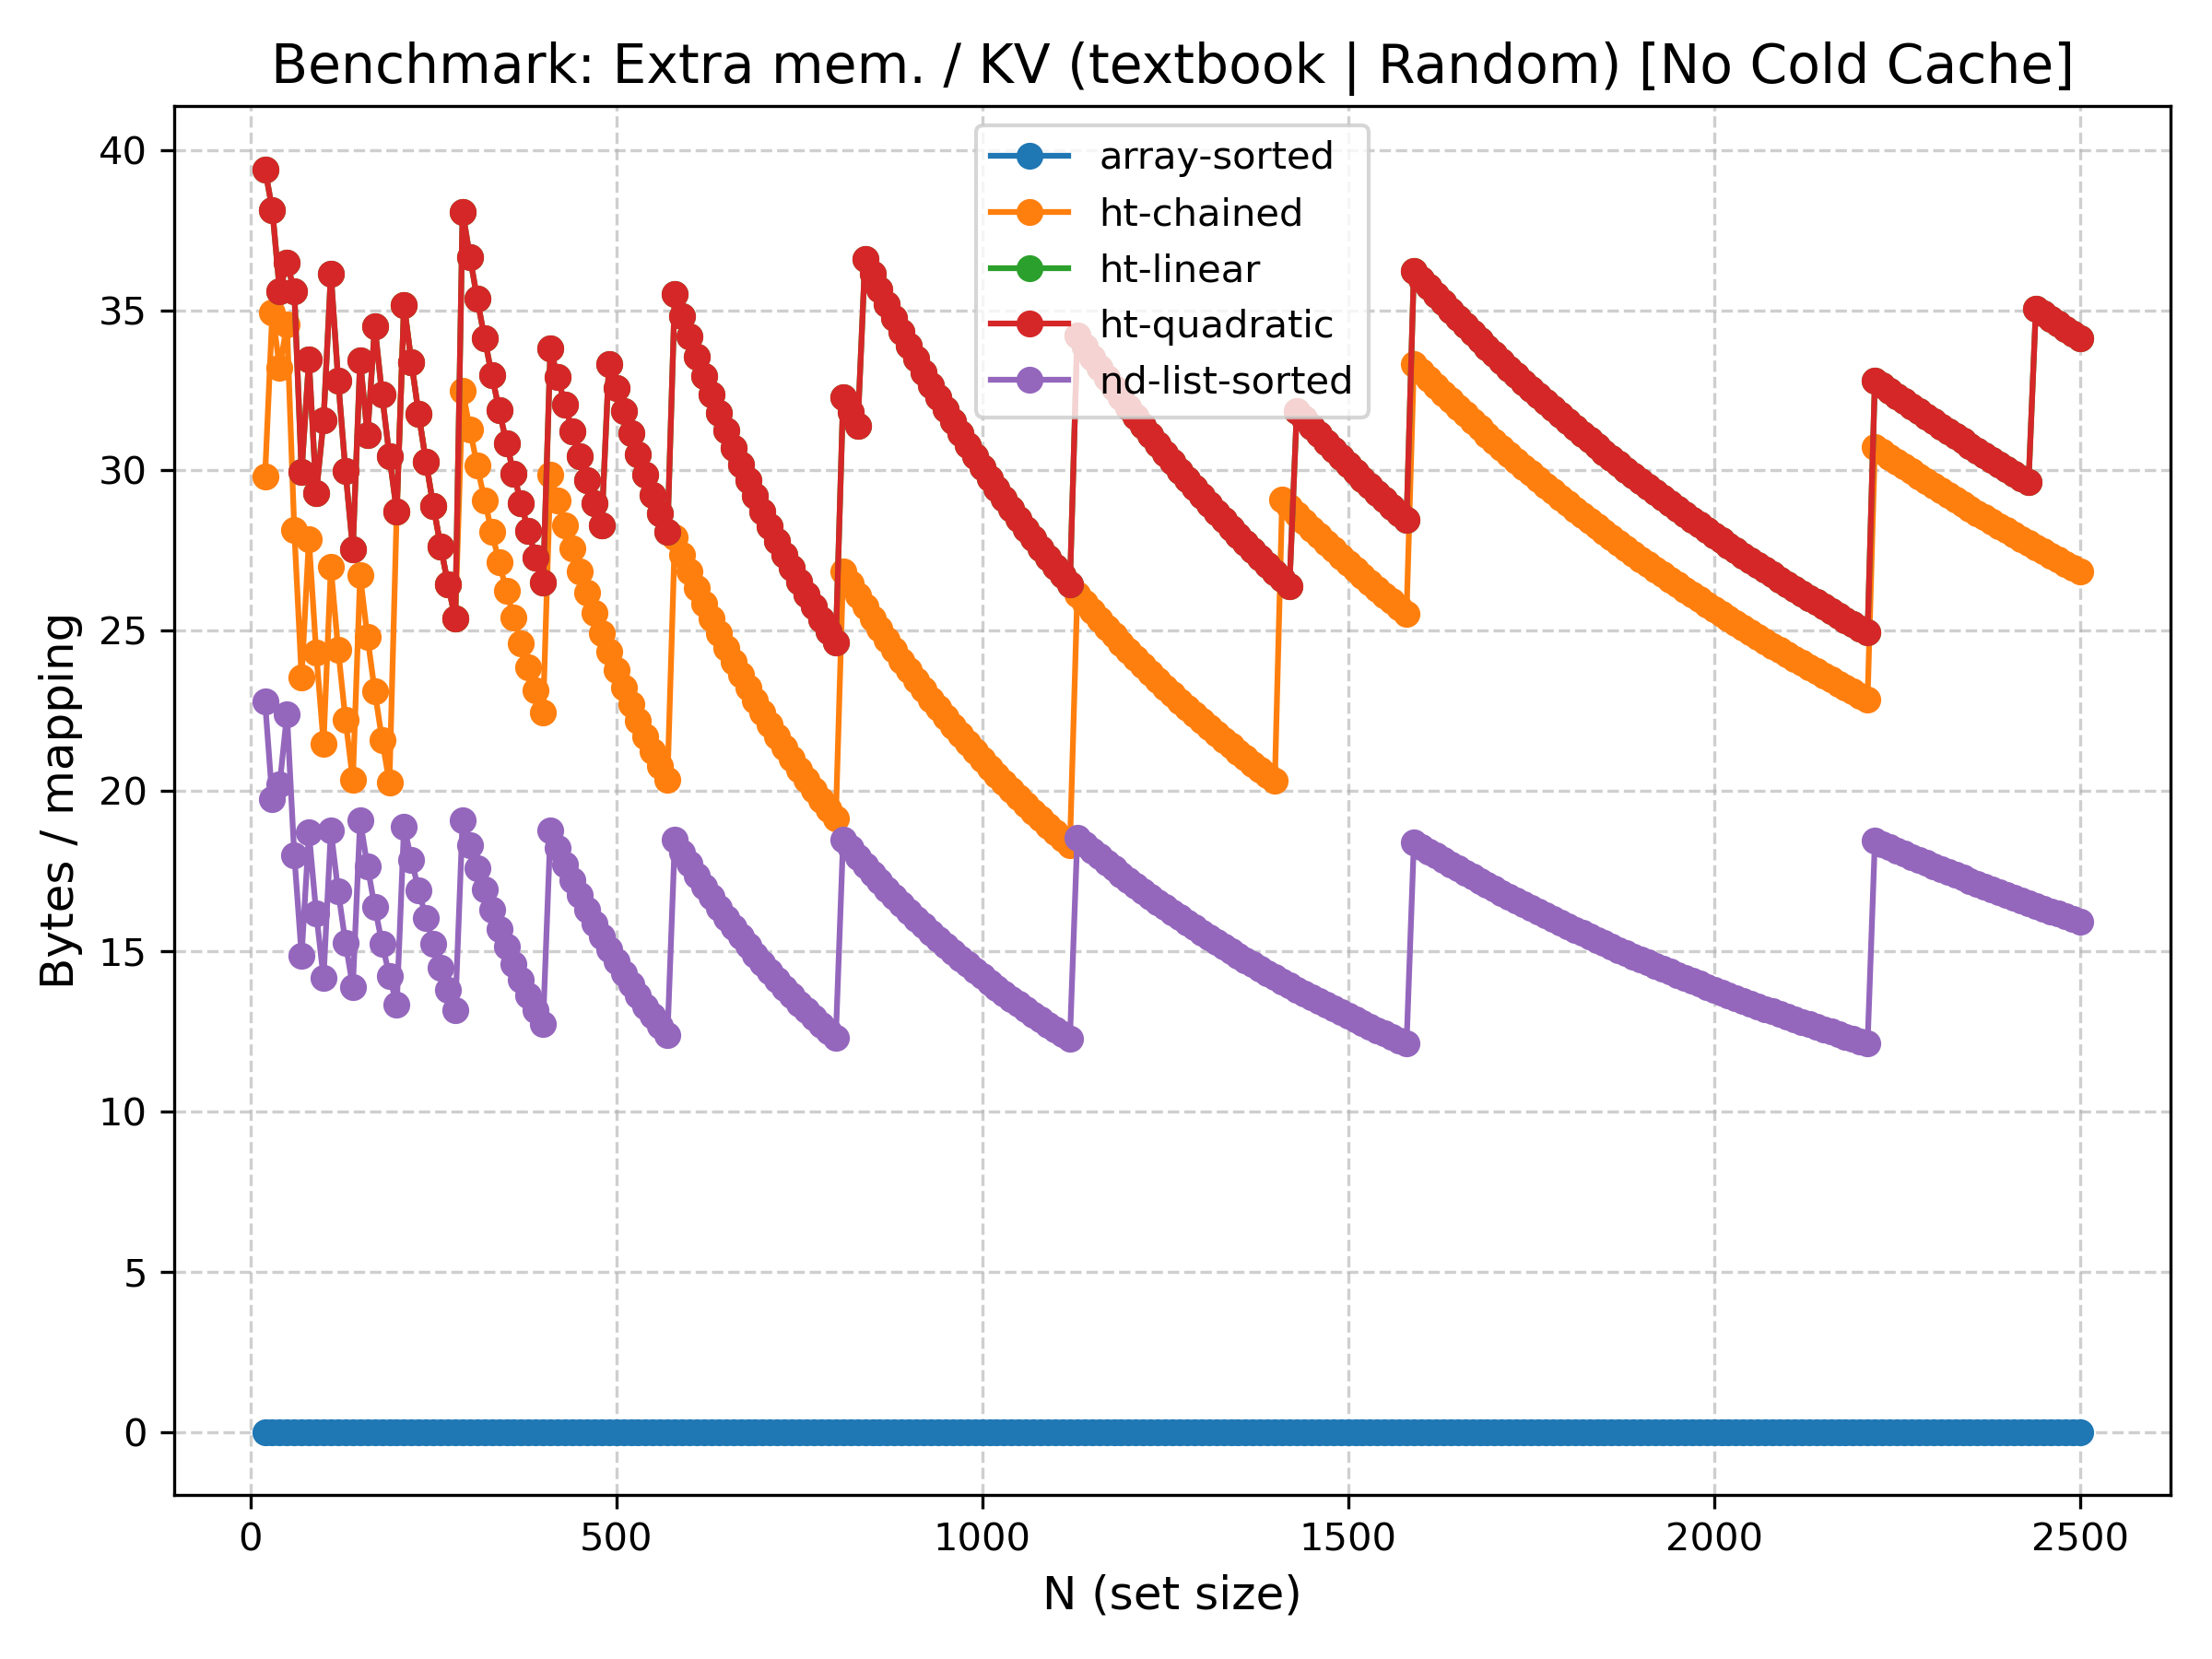
\includegraphics[scale=.3]{fig/plot_mem_nocold_abpkv.png}
  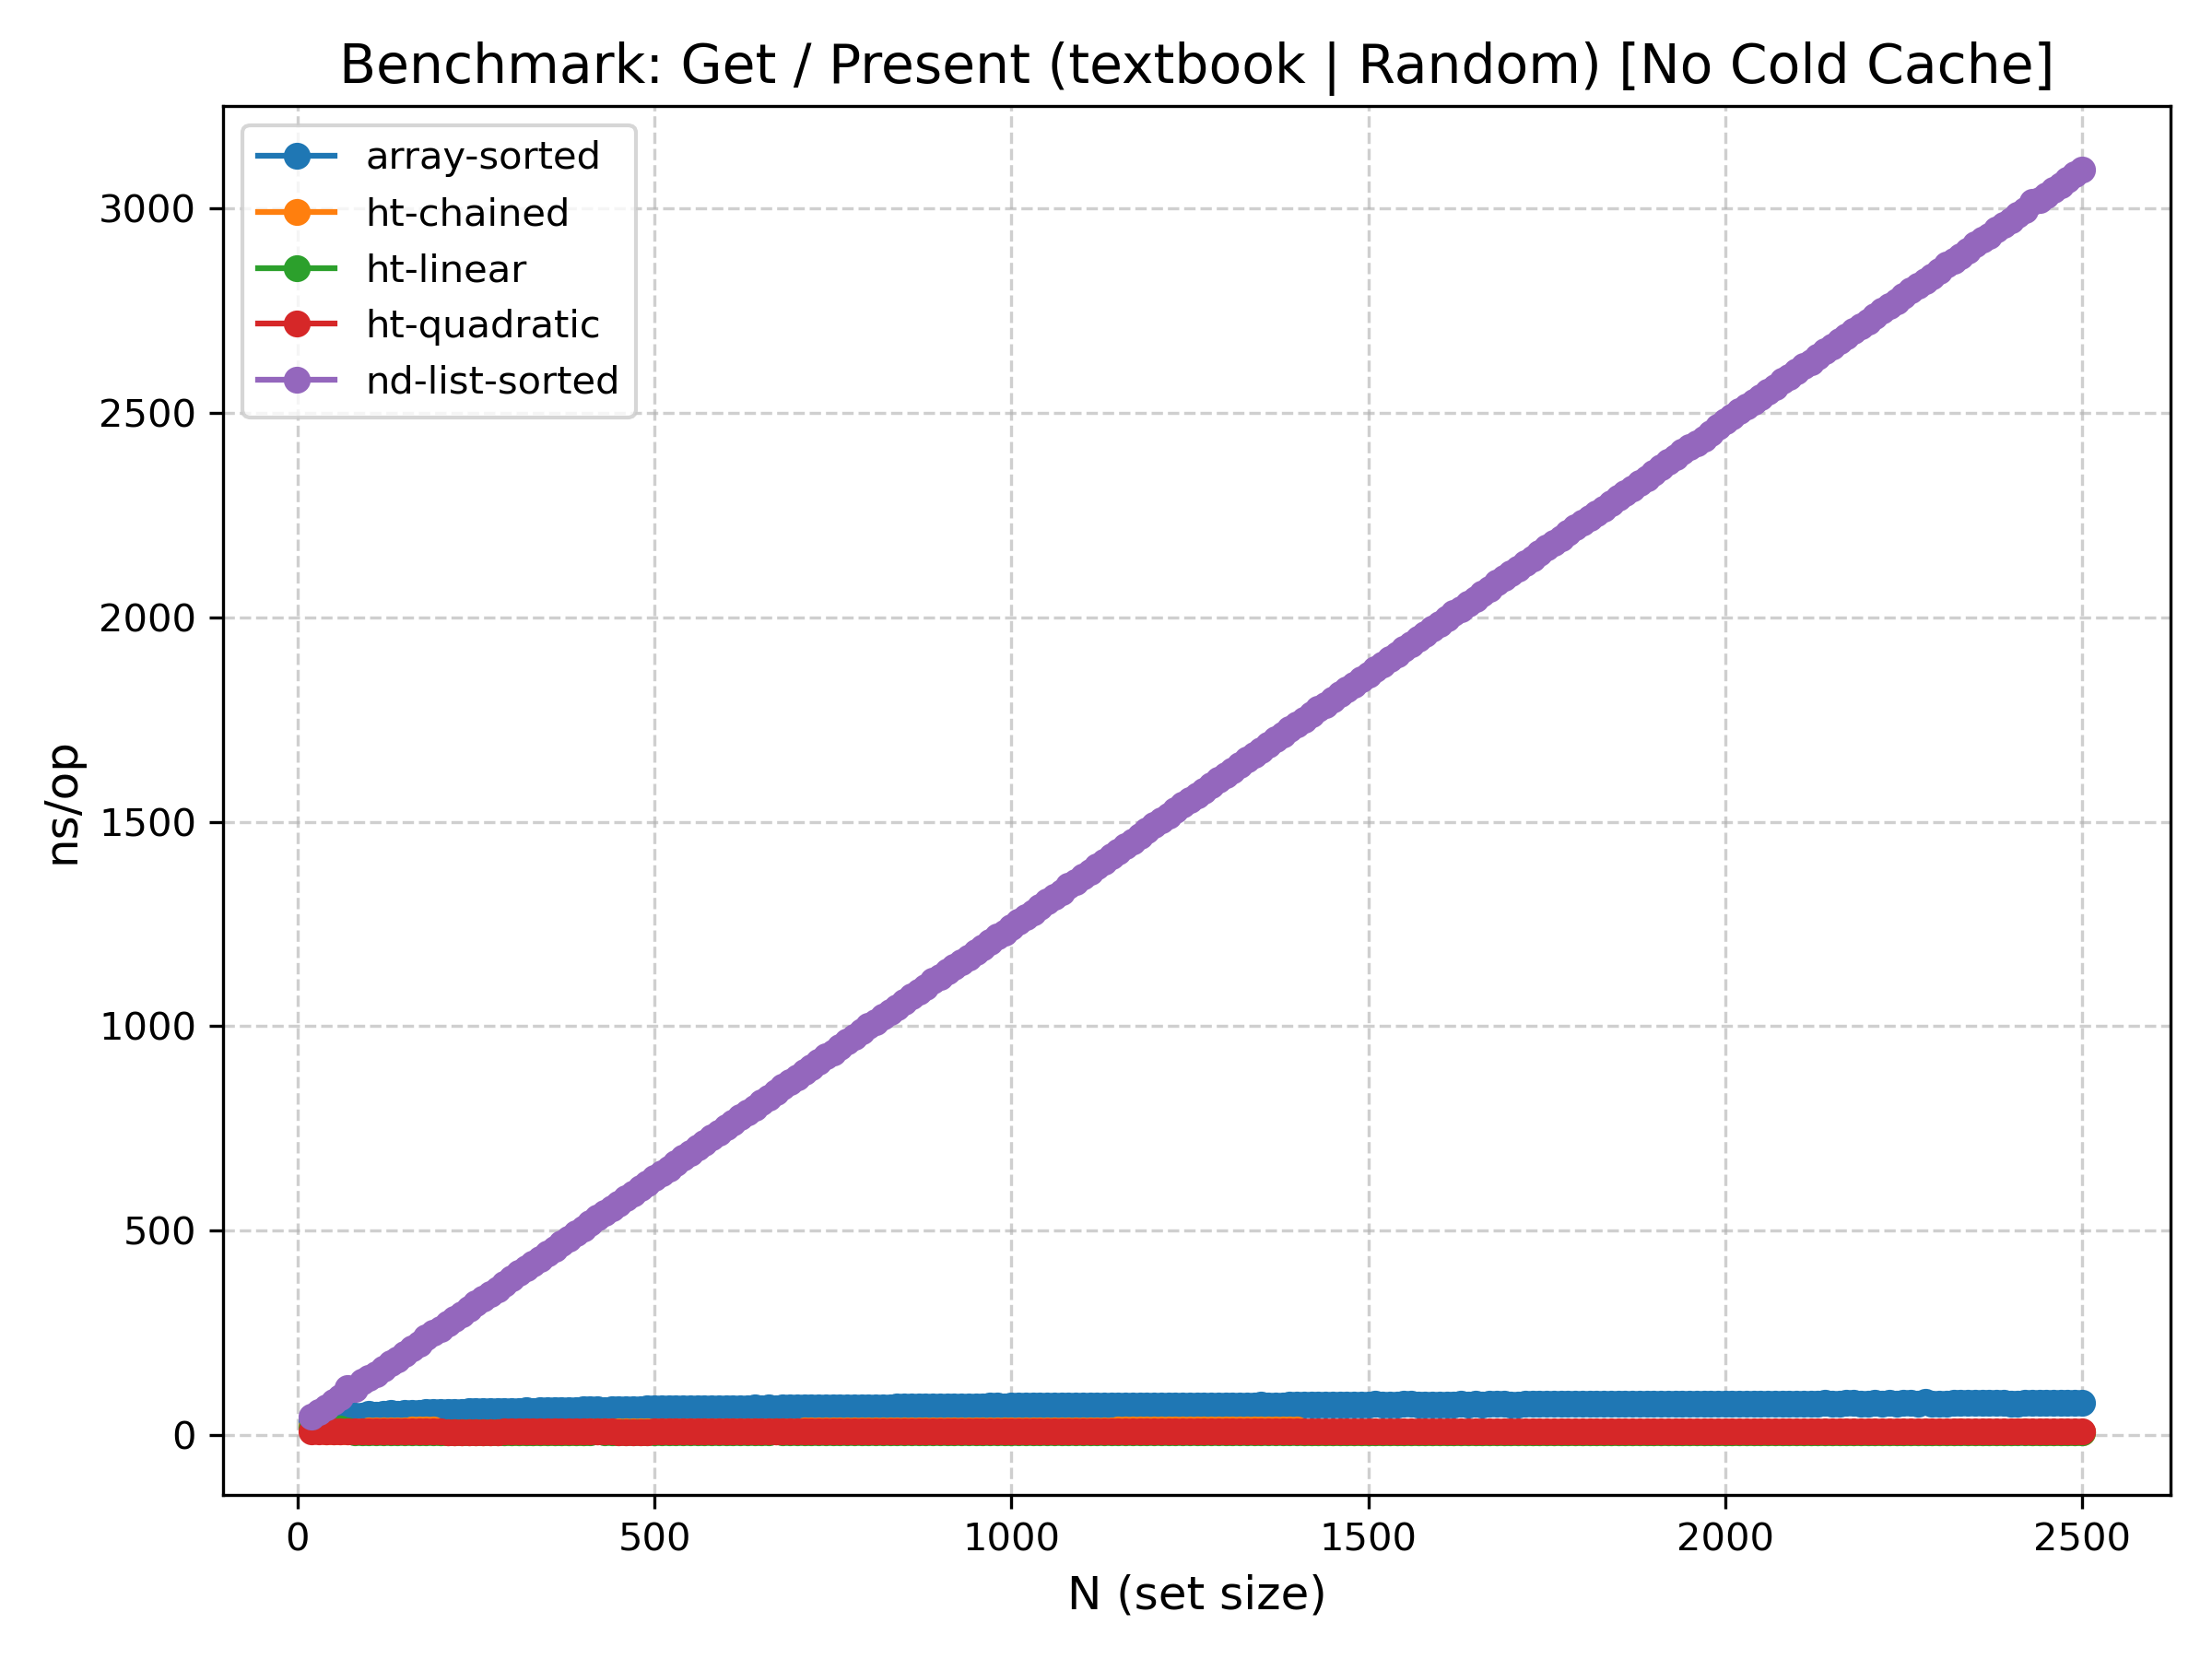
\includegraphics[scale=.3]{fig/plot_time_nocold_get_present.png}
\end{center}

\begin{itemize}
\item Once you've explained these plots and you're convinced linear-time is unusable:
  \begin{enumerate}
  \item Remove directory \lstinline{experiment/textbook/output} (or rename it to keep it.)

  \item Remove \lstinline{textbook-nd-list-sorted} from \lstinline{experiment/textbook/benchmark}
  \item Use more data: \lstinline{apman$ ./maplab --experiment textbook --preset small}
    
  \end{enumerate}
\end{itemize}

\end{frame}


% ----------------------------------------------------------------------
\begin{frame}[fragile]{\lstinline{apman$ ./maplab --experiment textbook --preset tiny} (cont'd)}

  For the radar plot: outer is better, solid line is median, shaded area is IQR.
  
\begin{center}
  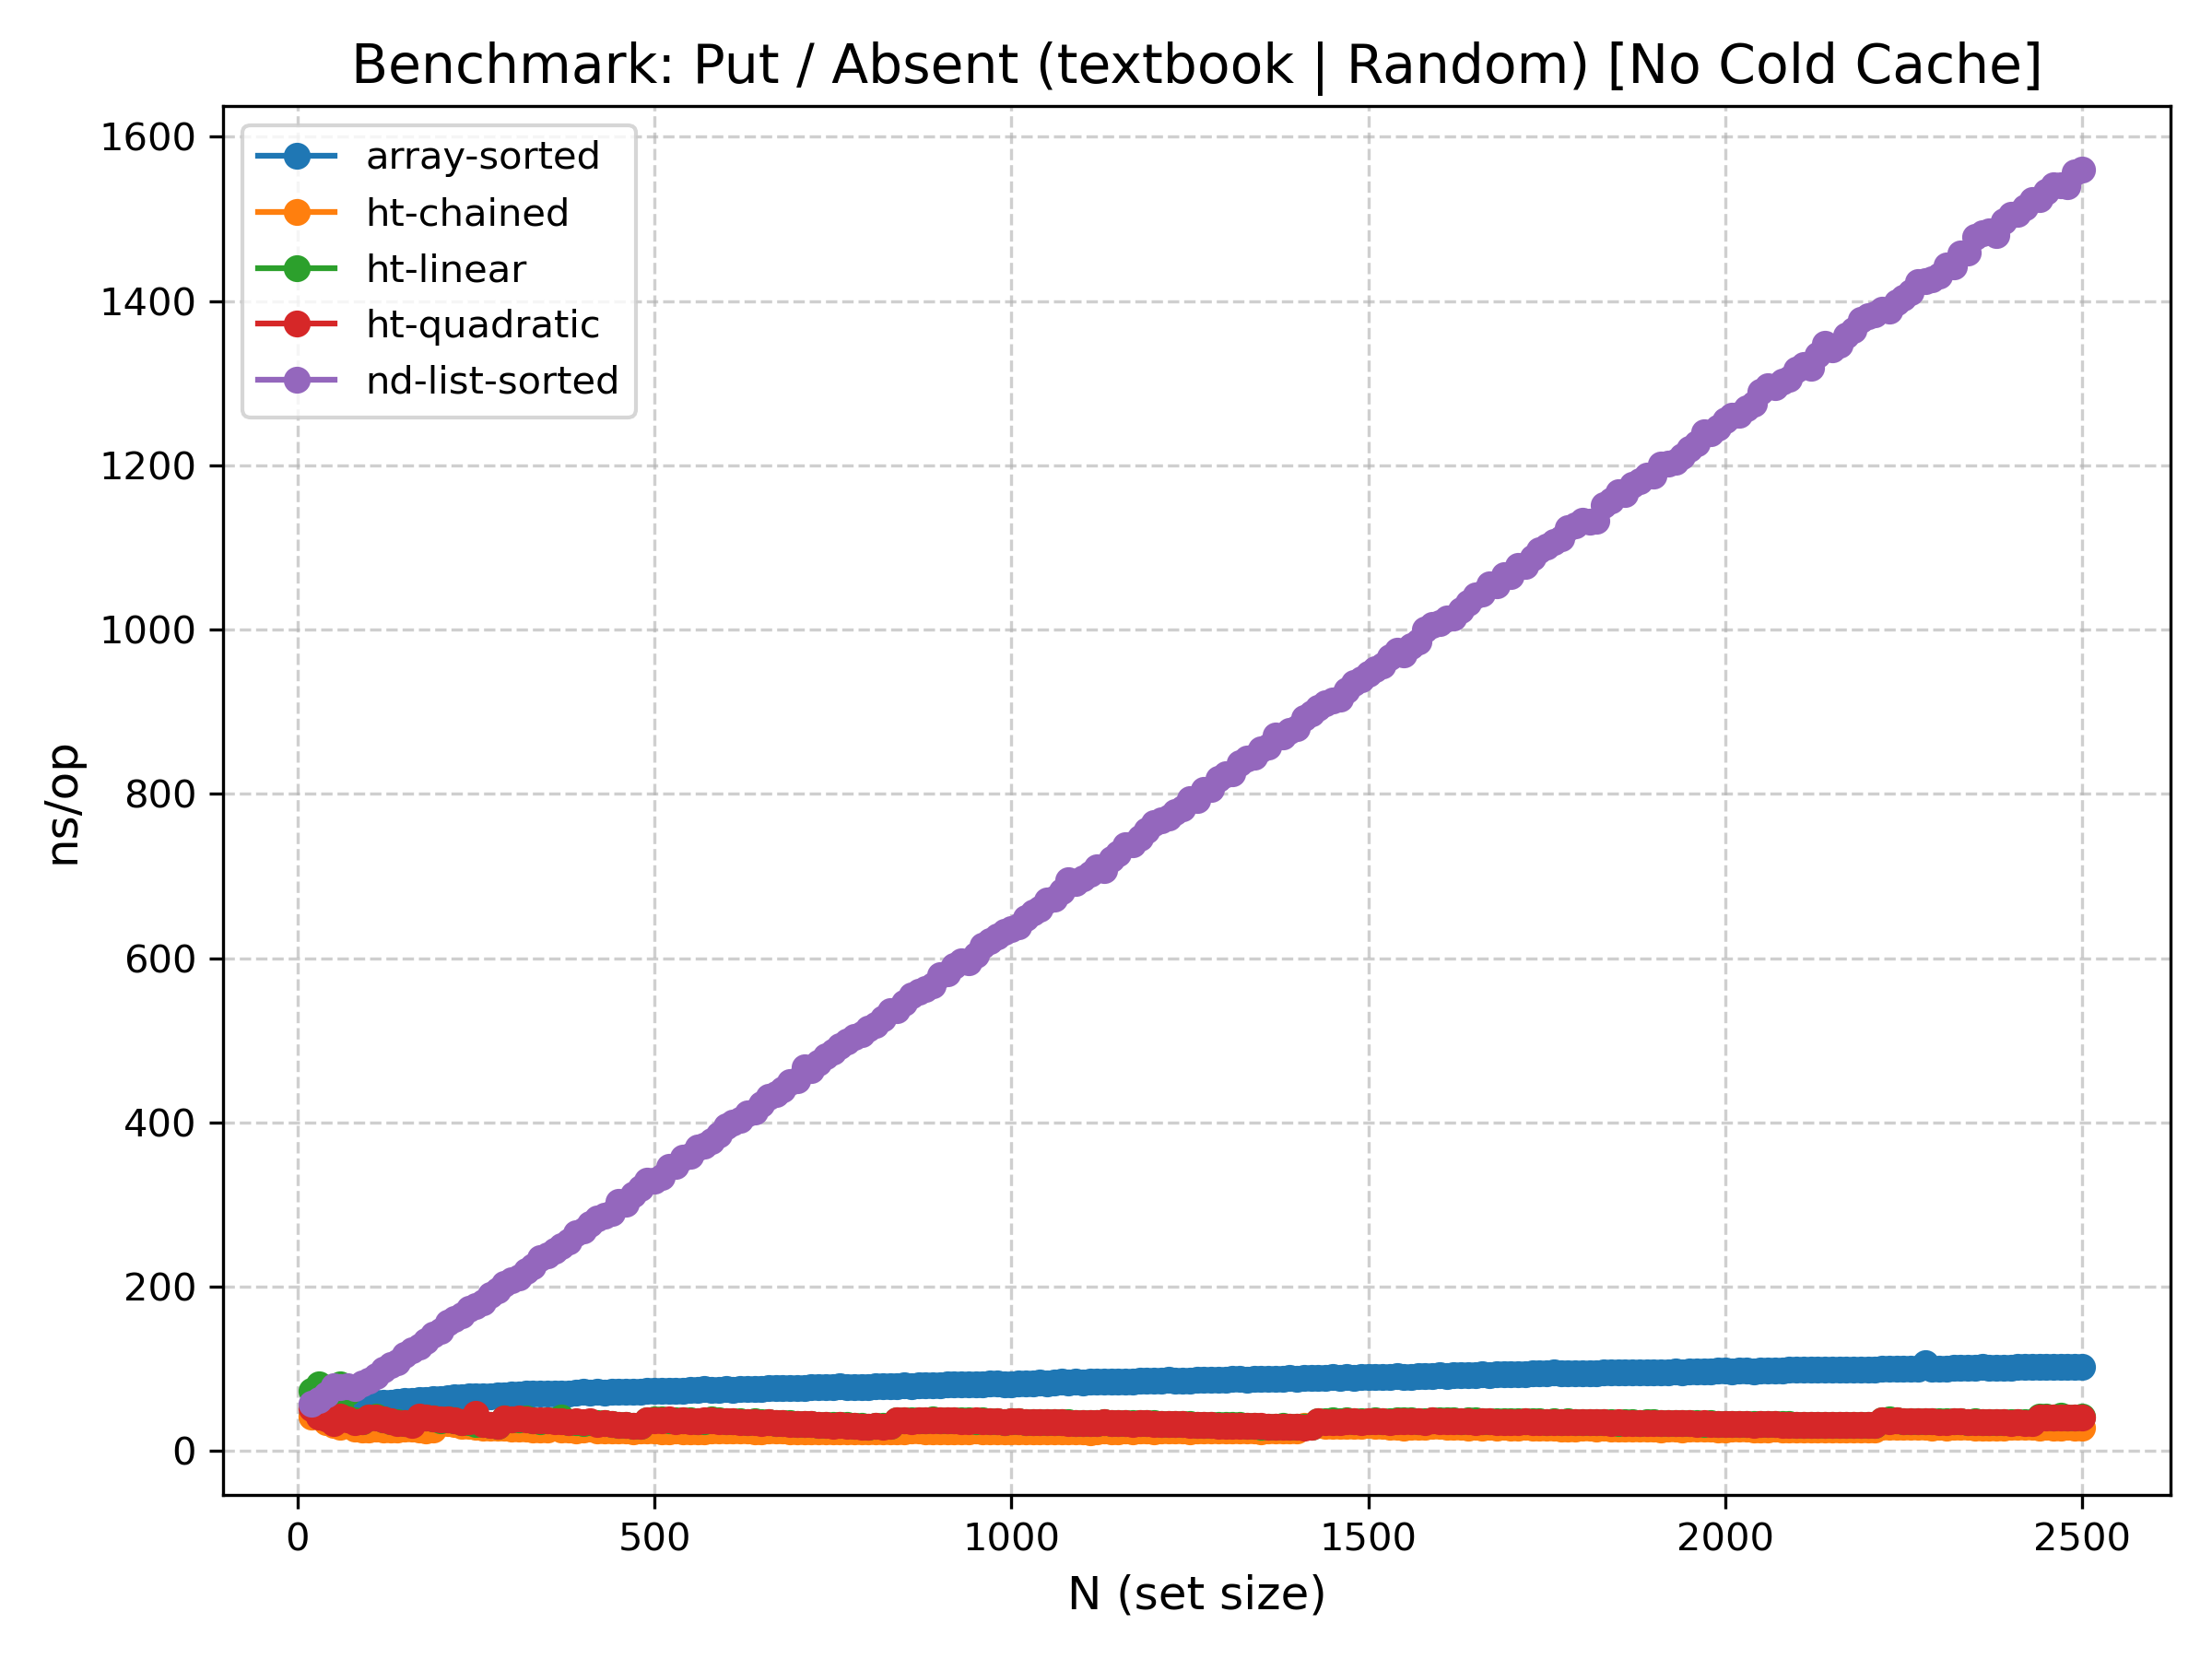
\includegraphics[scale=.3]{fig/plot_time_nocold_put_absent.png}
  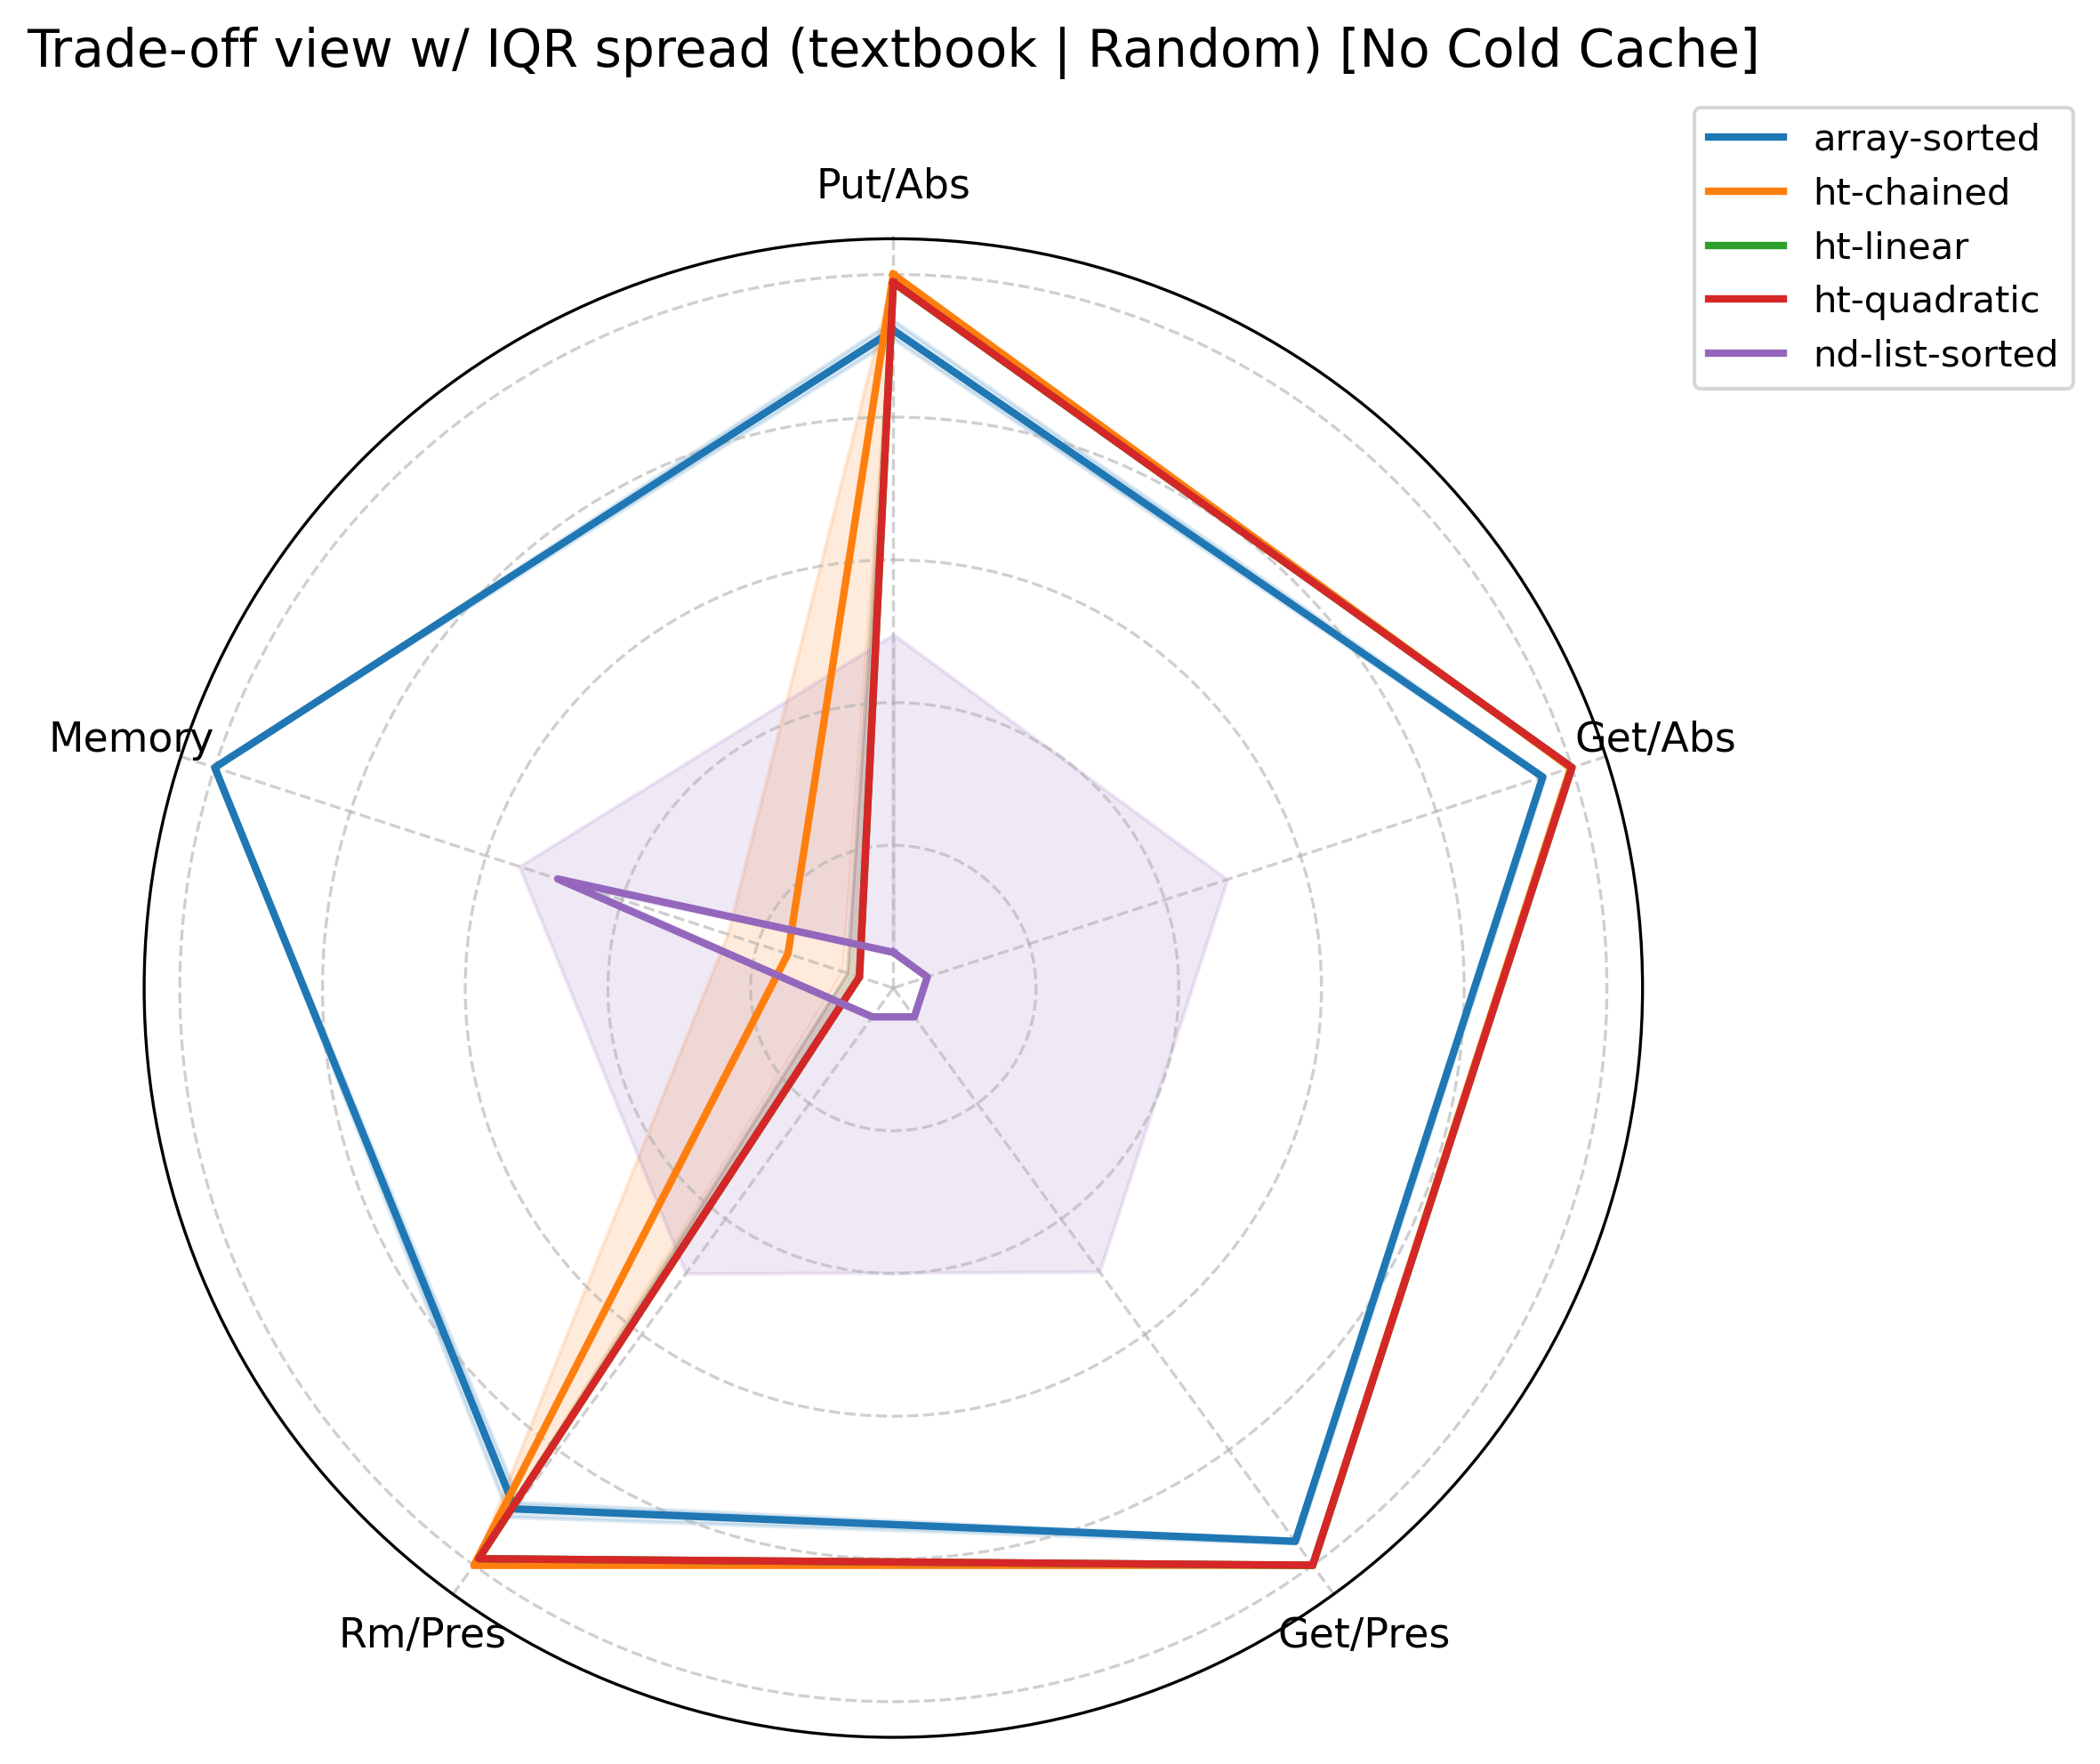
\includegraphics[scale=.3]{fig/radar_nocold_tradeoff.png}
\end{center}

\begin{itemize}
\item With options \lstinline{ds_secure_removal}, \lstinline{ds_ht_primes}, \lstinline{hash_no_finalize}, \lstinline{ds_ht_modulo_fast}, \texttt{ds\_ht\_lf\_\{min,max\}} already implemented, you can exercise benchmarking to draw a number of conclusions {\em today}.
\end{itemize}

\end{frame}


% ----------------------------------------------------------------------
\begin{frame}[fragile]{Maps}

  Learn how to {\em use} the environment and the methodology first.

  All while concentrating on implementing your best maps. In higher-level C.

  That should account for up to 70\% of the project.
  
  \begin{enumerate}
  \item Implement, test and benchmark map variants in:

    \texttt{include/ds/map/backend/\{chained,linear,quadratic,bst,hashtrie\}.h}
    
    This part of your report will basically be a plain textbook on algorithms.

    Your report should ask and answer the right questions with empirical evidence.

    See the \lstinline{README.md} for how to design and run map experiments.
    
  \item Download some real serious external code

    {\em Integrate} it in the benchmarks, {\em as seamlessly as possible}. Explain how you did.
    
    Give the wonderful {\em Verstable} map a try!

    Quadratic addressing with coalesced chains and {\em relative} pointers\dots

    Exercise your skills in C templating. You're only a couple \lstinline{#define}'s away!

  \end{enumerate}

  Those two steps ensure you master the coding standards at a reasonable level.
  
\end{frame}


% ----------------------------------------------------------------------
\begin{frame}[fragile]{Maps (cont'd)}

  You may also want to reflect on the methodology itself:
  
  \begin{enumerate}
  \item Feel free to dissect, criticize, evolve the tests or the benchmark

    Explain why and how you did (also to validate your approach.)

    For example, the benchmark cannot measure the effect of Move-to-Front.

    Also, the unit tests could be slightly more stringent. 

  \item Same for the map code

    You may want to handle insertion order more thoroughly (tombstones.)

    Also, it lacks proper de/allocation for the \lstinline{control} bytes!

  \end{enumerate}

\end{frame}


% ----------------------------------------------------------------------
\begin{frame}[fragile]{Add more (simpler!) data structures}

  \begin{enumerate}
  \item Add the {\em deque} data structure:
    \begin{itemize}
    \item Backends: resizable arrays {\em vs.} intrusive links (see)
    \item Upstream abstract data types: lists, stacks, queues
    \item Design the interface, the implementations, the tests and the benchmarks
    \item Explain the typical use cases.
    \end{itemize}

  \item {\em Embedded specials}
    \begin{itemize}
    \item Add a bip-buffer! Explain why it may be useful.
    \item Consider the resemblance with a general arena allocator\dots
    \item Map-related: implement Cuckoo hashing
    \end{itemize}
    
  \end{enumerate}

  Once you've followed the OS course, think of adding:
  \begin{itemize}
  \item A thread pool;
  \item Asynchronous computations with \lstinline{future_t}'s
  \item You may then start diving into the harsh world of {\em concurrent} data structures\dots
  \end{itemize}
  
\end{frame}


% ----------------------------------------------------------------------
\begin{frame}[fragile]{Typical report outline}

  A report skeleton is given in \lstinline{doc/report}.
  \begin{itemize}
  \item Pay attention to the many references you may want to explore!
  \end{itemize}

  We expect a discussion of the following points, backed by benchmarks where relevant:
  \begin{enumerate}
  \item Genericity: why and how?
  \item Arrays: why and how?
  \item Maps on unsorted data
    \begin{itemize}
    \item Hashtables
    \item Hashtries
    \end{itemize}
  \item Maps on sorted data
    \begin{itemize}
    \item Search trees
    \item Binary search
    \end{itemize}
  \item Deques
    \begin{itemize}
    \item Design of the data structure, of the tests, and of the benchmark
    \item Discussion of the sentinel technique for the link-based backend
    \end{itemize}
  \end{enumerate}

\end{frame}


% ----------------------------------------------------------------------
\begin{frame}[fragile]{What {\em we} will pay attention to}

  For example: 
  \begin{itemize}
  \item Could your report be used as a reference for other students?
  \item Quality, coverage, and validation/refutation of your hypotheses (maps)
  \item How the techniques we introduced were adapted (deques)
  \end{itemize}

  We show you a (vast) landscape, show us how you explore it scientifically!
  
\end{frame}




% ----------------------------------------------------------------------
\end{document}
